\documentclass{article}
\usepackage[left=4cm, right=3cm, top=3cm, bottom=3cm]{geometry}
\usepackage{amsmath}
\usepackage[hidelinks]{hyperref}
\DeclareMathOperator*{\argmax}{\arg\!\max}
\usepackage{amssymb}
\usepackage[utf8]{inputenc}
\usepackage{graphicx}
\graphicspath{{../images/}}
\usepackage{csquotes}
\usepackage[font={small, it}]{caption}

\title{Notes \\ Reinforcement Learning: An Introduction (2\textsuperscript{nd} Edition)}
\author{Scott Jeen}
\date{\today}

\begin{document}
	
\maketitle
\tableofcontents
\section{Introduction }	
\subsection{Overview}
\begin{itemize}
	\item Supervised learning = learning with labels defined by human; Unsupervised learning = finding patterns in data. Reinforcement learning is a 3rd machine learning paradigm, in which the agent tries to maximise its reward signal.
	\item Exploration versus exploitation problem - agent wants to do what it has already done to maximise reward by exploitation, but there may be a bigger reward available if it were to explore.
	\item RL is based on the model of human learning, similar to that of the brain's reward system.
\end{itemize}

\subsection{Elements of Reinforcement Learning}
\begin{description}
	\item[Policy] Defines the agent's way of behaving at any given time. It is a mapping from the perceived states of the environment to actions to be taken when in those states.
	\item[Reward Signal] The reward defines the goal of the reinforcement learning problem. At each time step, the environment sends the RL agent a single number, a \textit{reward}. It is the agent's sole objective to maximise this reward. In a biological system, we might think of rewards as analogous to pain and pleasure. The reward sent at any time depends on the agent's current action and the agent's current state. If my state is hungry and I choose the action of eating, I receive positive reward.
	\item[Value function] Reward functions indicate what is good immediately, but value functions specify what is good in the long run. The value function is the total expected reward an agent is likely to accumulate in the future, starting from a given state. E.g. a state might always yield a low immediate reward, but is normally followed by a string of states that yield high reward. Or the reverse. Rewards are, in a sense, primary, whereas values, as predictions of rewards, are secondary. Without rewards there could be no value. Nevertheless, it is values with which we are most concerned when evaluating decisions. We seek actions that bring the highest value, not the highest reward, because they obtain the greatest amount of reward over the long run. Estimating values is not trivial, and efficiently and accurately estimating them is the core of RL.
	\item[Model of environment (optionally)] Something that mimics the behaviour of the true environment, to allow inferences to be made about how the environment will behave. Given a state and action, the model might predict the resultant next state and next reward. They are used for \textit{planning}, that is, deciding on a course of action by considering possible future situations before they are actually experienced. 
\end{description}

	
	
	
	

\section{Multi-arm Bandits}

RL evaluates the actions taken rather than instructs correct actions like other forms of learning.

\subsection{An n-Armed Bandit Problem}
\textbf{The problem}
\begin{itemize}
\item You are faced repeatedly with a choice of \textit{n} actions.
\item After each choice, you receive a reward from a stationary probability distribution.
\item Objective is to maximise total reward over some time period, say 100 time steps.
\item Named after of slot machine (one-armed bandit problem), but \textit{n} levers instead of 1.
\item Each action has an expected or mean reward based on its probability distribution. We shall call thjs the \textit{value} of the action. We do not know these values with certainty.
\item Because of this uncertainty, there is always an exploration vs exploitation problem. We always have one action that we deem to be most valuable at any instant, but it is highly likely, at least initially, that there are actions we are yet to explore that are more valuable.
\end{itemize}

\subsection{Action-Value Methods}
The estimated action value is
\begin{equation} \label{eq: estimated value}
	Q_t(a) = \frac{R_1+R_2+\cdots+R_{N_t(a)}}{N_t(a)}
\end{equation}

The true value (mean reward) of an action is \(q\), but the estimated value at the \textit{t}th time-step is Q(a), given by Equation \ref{eq: estimated value} (our estimate after \textit{N} selections of an action yielding \textit{N} rewards).\\

The greedy action selection method is
\begin{equation} \label{eq: argmax}
A_t =\argmax_a Q_t(a)
\end{equation}

\begin{itemize}
	\item Simplest action selection rule is to select the action with the highest estimated value.
	\item $\argmax_a$ means the value of \(a\) for which \(Q_t\) is maximised.
	\item \(\epsilon\)-greedy methods are where the agent selects the greedy option most of the time, and selects a random action with probability \(\epsilon\).
	\item Three algorithms are tried: one with \(e\)=0 (pure greedy), one with \(e\)=0.01 and another with \(e\)=0.1
	\item Greedy method gets stuck performing sub-optimal actions.
	\item \(e\)=0.1 explores more and usually finds the optimal action earlier, but never selects it more that 91\% of the time.
	\item \(e\)=0.01 method improves more slowly, but eventually performs better than the e=0.1 method on both performance measures.
	\item It is possible to reduce \(e\) over time to try to get the best of both high and low values.
\end{itemize}
\begin{figure}
	\centering
	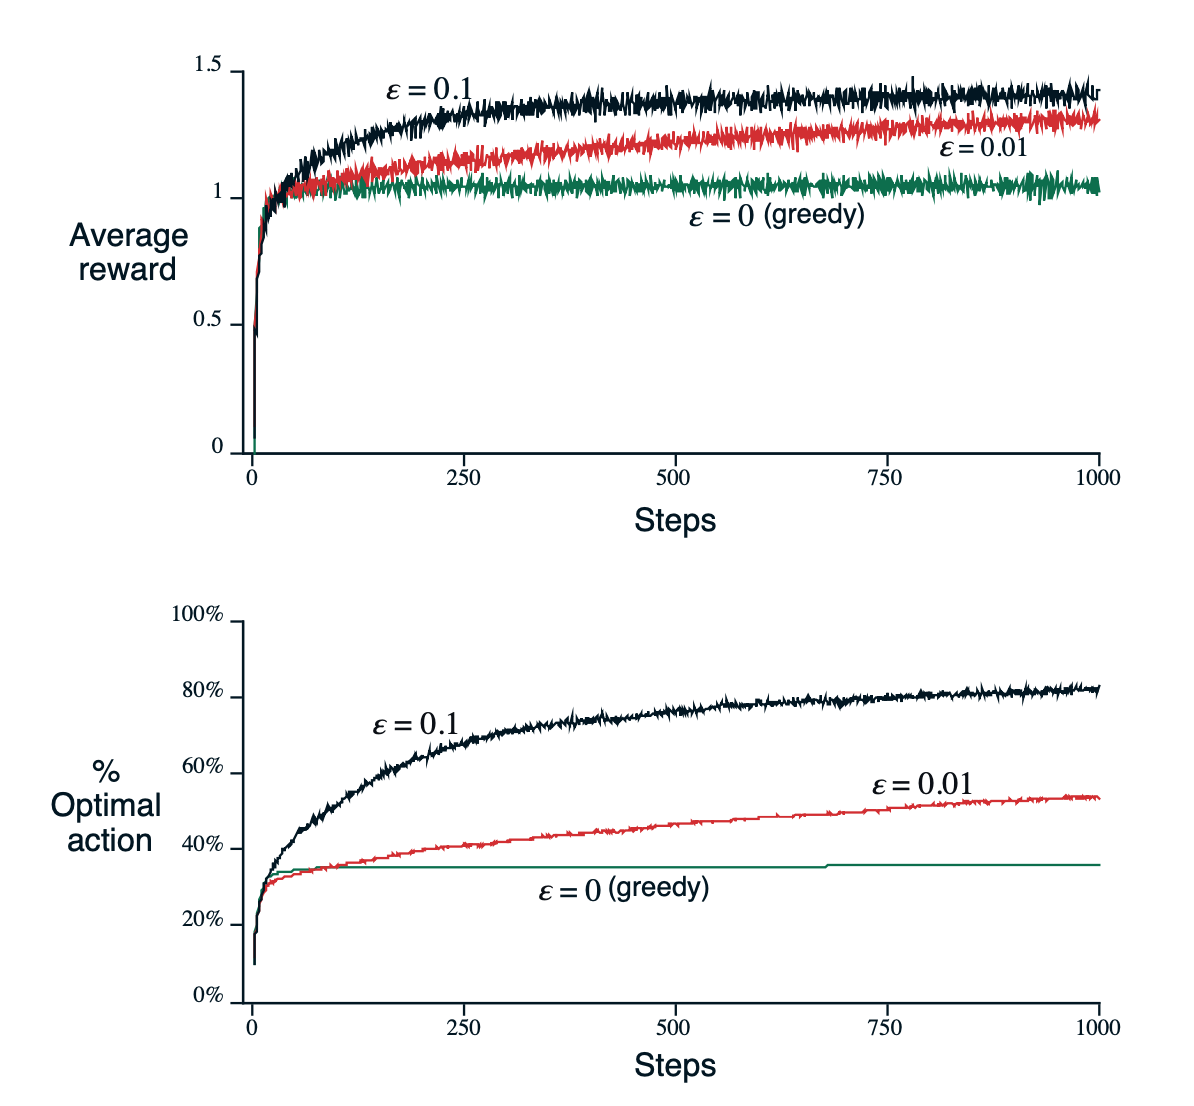
\includegraphics[width=0.8\textwidth]{/chapter2_1}
	\caption{Average performance of $\epsilon$-greedy action-value methods on the 10-armed testbed. These data are averages over 2000 runs with different bandit problems. All methods used sample averages as their action-value estimates.}
	\label{fig:chapter2_1}
\end{figure}

\subsection{Incremental Implementation}
The sample-average technique used to estimate action-values above has a problem: memory and computation requirements grow over time. This isn't necessary, we can devise an incremental solution instead:

\begin{align}
	Q_{k+1} &= \frac{1}{k}\sum_{i}^{k}R_i \nonumber \\
	&= \frac{1}{k} \left( R_k + \sum_{i=1}^{k-1} R_i \right) \nonumber \\
	&= \vdots \\
	&= Q_k + \frac{1}{k} \left[R_k - Q_k\right] \\
\end{align}

We are updating our estimate of \(Q_{k+1}\) by adding the discounted error between the reward just received and our estimate for that reward \(Q_k\).

\begin{equation}
NewEstimate \leftarrow OldEstimate + StepSize \left[Target - OldEstimate \right]
\end{equation}

\(\alpha\) is used to denote the stepsize (\(\frac{1}{k}\)) in the rest of this book.

\subsection{Tracking a Nonstationary Problem}
The averaging methods discussed above do not work if the bandit is changing over time. In such cases it makes sense to weight recent rewards higher than long-past ones. The popular way of doing this is by using a constant step-size parameter.

\begin{equation}
	Q_{k+1} = Q_k +\alpha \left[R_k - Q_k\right]
\end{equation}

where the step-size parameter \(\alpha \in (0,1]\) is constant. This results in \(Q_{k+1}\) being a weighted average of the past rewards and the initial estimate \(Q_1\):

\begin{align}
Q_{k+1} &= Q_k +\alpha \left[R_k - Q_k\right] \nonumber \\
&= \alpha R_k + (1 - \alpha)Q_k \nonumber \\
&= \alpha R_k + (1 - \alpha)[\alpha R_{k-1} + (1 - \alpha)Q_{k-1}] \nonumber \\
&= \alpha R_k + (1 - \alpha)\alpha R_{k-1} + (1 - \alpha)^2 Q_{k-1}  \nonumber \\
&= \vdots \nonumber \\
&= (1-\alpha)^k Q_1 + \sum_{i}^{k} \alpha (1 - \alpha)^{k-i} R_i \\
\end{align}

\begin{itemize}
\item Because the weight given to each reward depends on how many rewards ago it was observed, we can see that more recent rewards are given more weight. Note the weights \(\alpha\) sum to 1 here, ensuring it is indeed a weighted average where more weight is allocated to recent rewards.
\item In fact, the weight given to each reward decays exponentially into the past. This sometimes called an \textit{exponential} or \textit{recency-weighted} average.
\end{itemize}

\subsection{Optimistic Initial Values}
\begin{itemize}
\item The methods discussed so far are dependent to some extent on the initial action-value estimate i.e. they are biased by their initial estimates.
\item For methods with constant \(\alpha\) this bias is permanent.
\item In effect, the initial estimates become a set of parameters for the model that must be picked by the user.
\item In the above problem, by setting initial values to +5 rather than 0 we encourage exploration, even in the greedy case. The agent will almost always be disappointed with it's samples because they are less than the initial estimate and so will explore elsewhere until the values converge.
\item The above method of exploration is called \textit{Optimistic Initial Values}.
\end{itemize}

\subsection{Upper-confidence-bound Action Selection}
\(\epsilon\)-greedy action selection forces the agent to explore new actions, but it does so indiscriminately. It would be better to select among non-greedy actions according to their potential for actually being optimal, taking into account both how close their estimates are to being maximal and the uncertainty in those estimates. One way to do this is to select actions as:

\begin{equation}
	A_t = \argmax_a \left[Q_t(a) + c\sqrt{\frac{\ln t}{N_t(a)}}\right]
\end{equation}

where c \(>\) 0 controls the degree of exploration.

\begin{itemize}
	\item The square root term is a measure of the uncertainity in our estimate. It is proportional to \(t\) i.e. how many timesteps have passed and inversely proportional to \(N_t(a)\) i.e. how many times that action has been visited. The more time has passed, and the less we have sampled an action, the higher our upper-confidence-bound.
	\item As the timesteps increases, the denominator dominates the numerator as the ln term flattens.
	\item Each time we select an action our uncertainty decreases because N is the denominator of this equation.
	\item UCB will often perform better than e-greedy methods
\end{itemize}

\begin{figure}
	\centering
	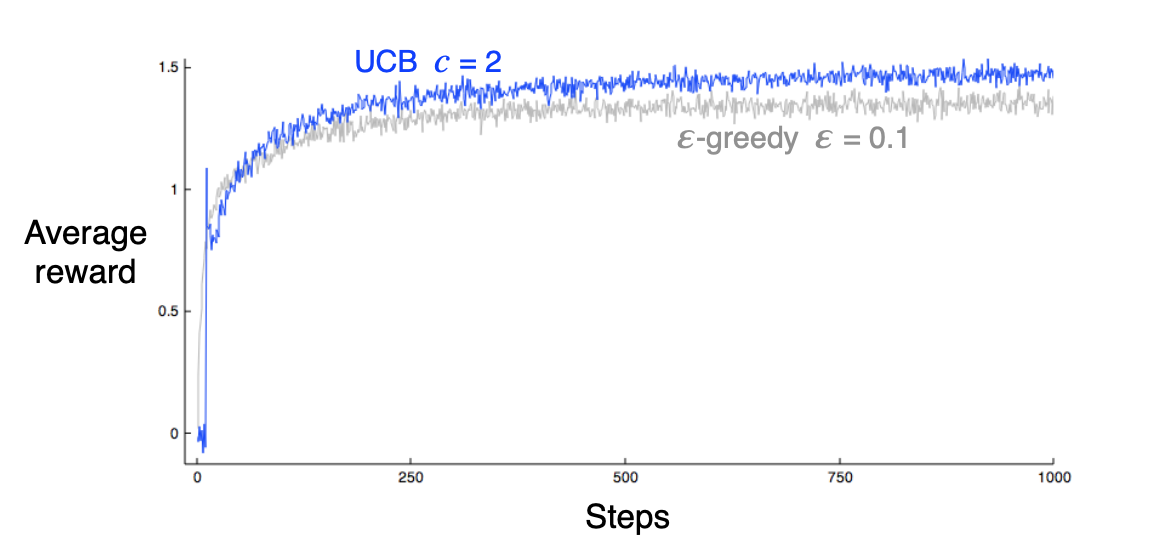
\includegraphics[width=0.8\textwidth]{/chapter2_2}
	\caption{UCB performs better than \(e\)-greedy in the n-armed bandit problem}
	\label{fig:chapter2_2}
\end{figure}

\subsection{Associative Search (Contextual Bandits)}
Thus far we have been discussing the stationary $k$-armed bandit problem, where the value of each arm is unknown but nonetheless remains stationary. Now, we consider a problem where the task could change from step to step, but the value distributions of the arms in each task remain the same. This is called contextual bandits, and in the toy example we are usually given a hint that the task has changed e.g. the slot machine changes colour for each task. Now we want to learn the correct action to take in a particular setting, given the task colour observed. This is an intermediary between the stationary problem and the full reinforcement learning problem. See exercise 2.10 below.

\subsection{Key Takeaways}
\begin{itemize}
\item The value of an action can be summarised by \(Q_t(a)\), the sample average return from an action
\item When selecting an action, it is preferable to maintain exploration, rather than only selecting the action we believe to be most valuable at any given timestep, to ensure we continue to improve our best estimate of the optimal action. We do so using \(\epsilon\))-greedy policies.
\item If our problem is non-stationary, rather than taking a standard average of every return received after an action, we can take a weighted average that gives higher value to more recently acquired rewards. We call this an \textit{exponential} or \textit{recency-weighted} average.
\item Optimistic initial values encourage lots of early exploration as our returns always decrease our estimate of \(Q_t\) meaning the greedy actions remain exploratory. Only useful for stationary problems.
\item \(\epsilon\)-greedy policies can be adapted to give more value to actions that have been selected less-often, i.e. actions where we have higher uncertainty in their value, using \textit{upper-confidence-bound} action selection.
\item Lastly, each of these techniques have varied performance on the n-armed bandit test dependent on their parametrisation. Their performance is plotted in Figure \ref{fig:chapter2_4}.
\end{itemize}

\begin{figure}
	\centering
	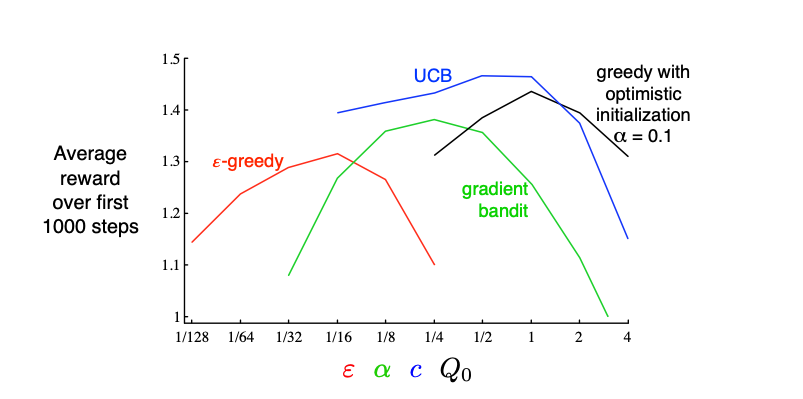
\includegraphics[width=0.8\textwidth]{/chapter2_4}
	\caption{Performance of each of the bandit algorithms explored in this chapter}
	\label{fig:chapter2_4}
\end{figure}


\section{Finite Markov Decision Processes}

\subsection{The Agent-Environment Interface}
\begin{figure}[h!]
	\centering
	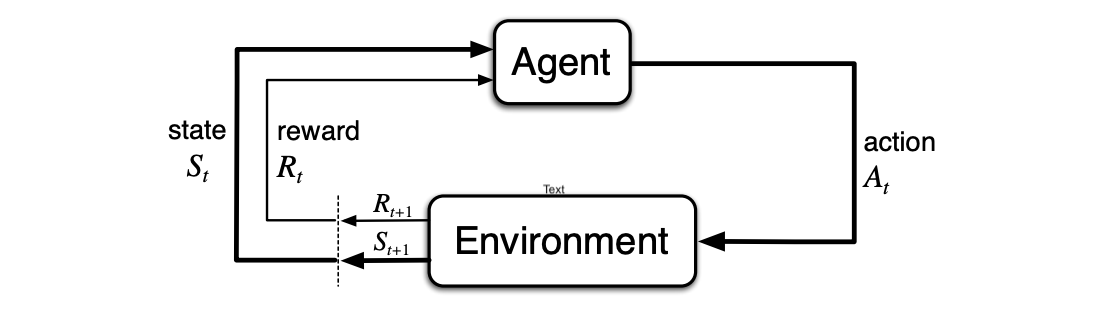
\includegraphics[width=\textwidth]{/chapter3_1}
	\caption{The agent-environment interface in reinforcement learning}
	\label{fig:agent-environment}
\end{figure}

\begin{itemize}
	\item At each timestep the agent implements a mapping from states to probabilities of selecting a possible action. The mapping is called the agents \textit{policy}, denoted \(\pi\), where \(\pi(a | s)\) is the probability of the agent selecting actions a in states.
	\item In general, actions can be any decision we want to learn how to make, and states can be any interpretation of the world that might inform those actions.
	\item The boundary between agent and environment is much closer to the agent than is first intuitive. E.g. if we are controlling a robot, the voltages or stresses in its structure are part of the environment, not the agent. Indeed reward signals are part of the environment, despite very possibly being produced by the agent e.g. dopamine.
\end{itemize}

\subsection{Goals and Rewards}
The \textit{reward hypothesis}:
\begin{displayquote}
	All we mean by goals and purposes can be well thought of as the maximization of the expected value of the cumulative sum of a received scalar signal (called reward).
\end{displayquote}

The reward signal is our way of communicating to the agent what we want to achieve not how we want to achieve it.

\subsection{Returns and Episodes}
The return \(G_t\) is the sum of future rewards:

\begin{equation}
	G_t = R_{t+1} + R_{t+2} + R_{t+3} + \cdots + R_t
\end{equation}

\begin{itemize}
	\item This approach makes sense in applications that finish, or are periodic. That is, the agent-environment interaction breaks into \textit{episodes}.
	\item We call these systems \textit{episodic tasks}. e.g playing a board game, trips through a maze etc.
	\item Notation for state space in an episodic task varies from the conventional case (\(s \in \mathcal{S}\)) to (\(s \in \mathcal{S^+}\))
	\item The opposite, continuous applications are called \textit{continuing tasks}.
	\item For these tasks we use \textit{discounted returns} to avoid a sum of returns going to infinity.
\end{itemize}

\begin{equation}
	G_t = R_{t+1} + \gamma R_{t+2} + \gamma^2 R_{t+3} + \cdots = \sum_{k=0}^{\infty} \gamma^k R_{t+k+1} 
\end{equation}

If the reward is a constant + 1 at each timestep, cumulative discounted reward $G_t$ becomes:

\begin{equation}
G_t = \sum_{k=0}^{\infty} \gamma^k = \frac{1}{1 - \gamma}
\end{equation}

\textit{Discounting} is a crucial topic in RL. It allows us to store a finite value of any state (summarised by its expected cumulative reward) for continuous tasks, where the non-discounted value would run to infinity. 

\subsection{Unified Notation for Episodic and Continuing Tasks}
\begin{equation}
	G_t = \sum_{k=0}^{T-t-1} \gamma^k R_{t+k+1} 
\end{equation}

\subsection{The Markov Property}
A state signal that succeeds in retaining all relevant information about the past is \textit{Markov}. Examples include:
\begin{itemize}
\item A cannonball with known position, velocity and acceleration
\item All positions of chess pieces on a chess board.
\end{itemize}

In normal causal processes, we would think that our expectation of the state and reward at the next timestep is a function of all previous states, rewards and actions, as follows:

\begin{equation}
	Pr \{R_{t+1} = r, S_{t+1} = s' | S_0, A_0, R_1, \ldots, S_{t-1}, A_{t-1}, R_t, S_t, A_t\}  
\end{equation}

If the state is Markov, however, then the state and reward right now completely characterizes the history, and the above can be reduced to:

\begin{equation}
p(s', r | s, a) = Pr \{R_{r+1} = r, S_{t+1} = s' | S_t, A_t\}
\end{equation}

\begin{itemize}
\item Even for non-Markov states, it is appropriate to think of all states as at least an approximation of a Markov state.
\item Markov property is important in RL because decisions and values are assumed to be a function only of the current state.
\item Most real scenarios are unlikely to be Markov. In the example of controlling HVAC, the HVAC motor might heat up which affects cooling power and we may not be tracking that temperature. It is hard for a process to be Markov without sensing all possible variables.
\end{itemize}

\subsection{Markov Decision Process (MDP)}
Given any state and action s and a, the probability of each possible pair of next state and reward, s', r is denoted:

\begin{equation}
p(s', r | s, a) = Pr \{R_{r+1} = r, S_{t+1} = s' | S_t, A_t\}
\end{equation}

We can think of \(p(s', r | s, a)\) as the dynamics of our MDP, often called the \textit{transition function}–it defines how we move from state to state given actions. 

\subsection{Policies and Value Functions}
\begin{itemize}
\item Value functions are functions of states or functions of state-value pairs.
\item They estimate how good it is to be in a given state, or how good it is to perform a given action in a given state.
\item Given future rewards are dependent on future actions, value functions are defined with respect to particular policies as the value of a state depends on the action an agent takes in said state.
\item A \textit{policy} is a mapping from states to probabilities of selecting each possible action.
\item RL methods specify how the agent's policy changes as a result of its experience.
\item For MDPs, we can define $v(\pi(s))$ formally as:
\end{itemize}

\begin{equation}
v_\pi(s) = \mathbb{E}_\pi \left[G_t | S_t = s \right] = \mathbb{E}_\pi \left[\sum_{k=0}^{\infty} \gamma^k R_{t+k+1} | S_t = s\right]
\end{equation}

i.e. the expected future rewards, given state \(S_t\), and policy \(\pi\). We call \(v_\pi(s)\)the \textit{state value function for policy} $\pi$. Similarly, we can define the value of taking action \(a\) in state \(s\) under policy \(\pi\) as:

\begin{equation}
q_\pi(s,a) = \mathbb{E}_\pi \left[G_t | S_t = s, A_t = a \right] = \mathbb{E}_\pi \left[\sum_{k=0}^{\infty} \gamma^k R_{t+k+1} | S_t = s, A_t = a \right]
\end{equation}

i.e. the expected value, taking action \(a\) in state \(s\) then following policy \(\pi\).
\begin{itemize}
\item We call \(q_\pi\) the \textit{action-value function for policy \(\pi\)}
\item Both value functions are estimated from experience.
\end{itemize}

A fundamental property of value functions used throughout reinforcement learning and dynamic programming is that they satisfy recursive relationships similar to that which we have already established for the return. This recursive relationship is characterised by the \textit{Bellman Equation}:

\begin{equation}
v_\pi(s) = \sum_{a} \pi(a|s) \sum_{s',r} p(s', r | s, a) \left[r + \gamma v_\pi(s')\right]
\end{equation}

This recursion looks from one state through to all possible next states given our policy and the dynamics as suggested by \ref{fig:backup}:
\begin{figure}[h!]
	\centering
	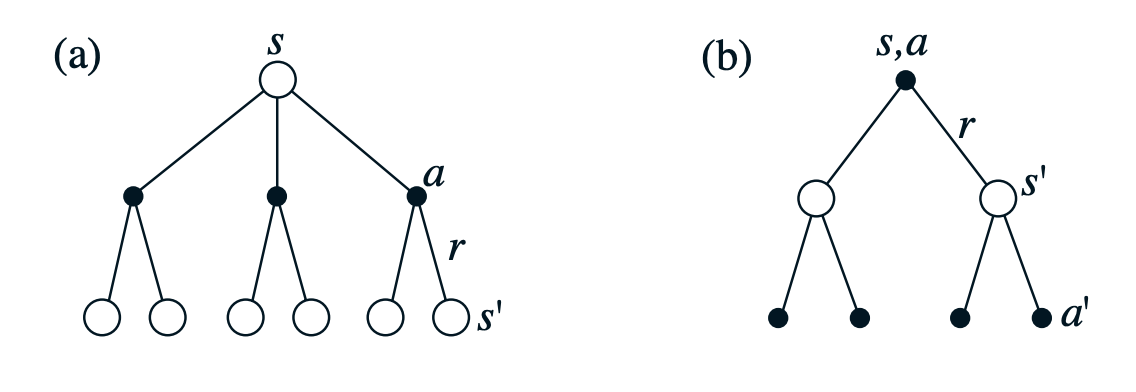
\includegraphics[width=\textwidth]{/chapter3_2}
	\caption{Backup diagrams for \(v_\pi\) and \(q_\pi\)}
	\label{fig:backup}
\end{figure}

\subsection{Optimal Policies and Value Functions}
\begin{itemize}
\item A policy \(\pi '\) is defined as better than policy pi if its expected return is higher for all states.
\item There is always \textit{at least} one policy that is better than or equal to all other policies - this is the \textit{optimal policy}.
\item Optimal policies are denoted \(\pi_*\)
\item Optimal state-value functions are denoted \(v_*\)
\item Optimal action-value functions are denoted \(q_*\)
\item We can write \(q_*\) in terms of \(v_*\):
\end{itemize}

\begin{equation}
q_*(s,a) = \mathbb{E} \left[R_{t+1} + \gamma v_*(S_{t+1}) | S_t = s, A_t = a \right]
\end{equation}

We can adapt the Bellman equation to achieve the Bellman optimality equation, which takes two forms. Firstly for \(v_*\):
\begin{equation}
v_*(s) = \max_{a \in \mathcal{A}(s)} \sum_{s',r} p(s', r | s, a) \left[r + \gamma v_*(s')\right]
\end{equation}
and secondly for \(q_*\):
\begin{equation}
q_*(s) = \sum_{s',r} p(s', r | s, a) \left[r + \gamma \max_{a'} q_*(s', a') \right]
\end{equation}

\begin{itemize}
\item Using \(v_*\) the optimal expected long term return is turned into a quantity that is immediately available for each state. Hence a one-step-ahead search, acting greedily, yield the optimal long-term actions.
\item Fully solving the Bellman optimality equations can be hugely expensive, especially if the number of states is huge, as is the case with most interesting problems.
\item Solving the Bellman optimality equation is akin to exhaustive search. We play out \textit{every} possible scenario until the terminal state and collect their expected reward. Our policy then defines the action that maximises this expected reward. 
\item In the continuous case the Bellman optimality equation is unsolvable as the recursion on the next state's value function would never end.
\end{itemize}

\subsection{Optimality and Approximation}
\begin{itemize}
	\item We must approximate because calculation of optimality is too expensive.
	\item A nice way of doing this is allowing the agent to make sub-optimal decisions in scenarios it has low probability of encountering. This is a trade off for being optimal in situations that occur frequently.
\end{itemize}

\subsection{Key Takeaways}
\begin{itemize}
\item We summarise our goal for the agent as a \textit{reward}; its objective is to maximise the cumulative sum of future rewards
\item For episodic tasks, returns terminate (and are backpropogated) when the episode ends. For the continuous control case, returns are discounted so they do not run to infinity. 
\item A state signal that succeeds in retaining all relevant information about the past is \textit{Markov}. 
\item Markov Decision Processes (MDPs) are the mathematically idealised version of the RL problem. They have system dynamics: $p(s', r | s, a) = Pr \{R_{r+1} = r, S_{t+1} = s' | S_t, A_t\}$
\item Policies are a (probabilistic) mapping from states to actions.
\item Value functions estimate how good it is for an agent to be in a state ($v_\pi$) or to take an action from a state ($q_\pi$). They are always defined w.r.t policies as the value of a state depends on the policy one takes in that state. Value functions are the \textit{expected cumulative sum of future rewards} from a state or state-action pair.
\item Knowing our policy and system dynamics, we can define the state value function is defined by the Bellman equation: $v_\pi(s) = \sum_{a} \pi(a|s) \sum_{s',r} p(s', r | s, a) \left[r + \gamma v_\pi(s')\right]$
\item An optimal policy ($\pi_*$) is the policy that maximises expected cumulative reward from all states. From the optimal policy we can derive the optimal value functions $q_*$ and $v_*$.
\end{itemize}











\section{Dynamic Programming}

\subsection{Policy Evaluation}
\begin{itemize}
\item Computing the value function for an arbitrary policy \(\pi\). Ideally, we would do this using dynamic programming if the state-space is finite and we know the state transition perfectly.
\end{itemize}


\subsection{Policy Improvement}
\begin{itemize}
\item Take our policy and associated value function obtained through policy evaluation. Then in state s, we take a different action `a` not prescribed by our policy, follow our normal policy thereafter, and see if the value function changes. If the value of that state improves then we say that our policy has improved.
\item If we extend this to the limit and choose to take the value-maximising action in each state we call this acting greedily with respect to our value function.
\end{itemize}


\subsection{Policy Iteration}
By flipping between policy evaluation and iteration we can achieve a sequence of monotonically increasing policies and value functions. Algorithm is:
\begin{enumerate}
\item Evaluate policy \(\pi\) to obtain value function \(V_\pi\)
\item Improve policy \(\pi\) by acting greedily with respect to \(V_\pi\) to obtain new policy \(\pi'\)
\item Evaluate new policy \(\pi'\) to obtain new value function `\(V_{\pi'}\)
\item Repeat until new policy is no longer better than the old policy, at which point we have obtained the optimal policy. (Only for finite MDPs)
\end{enumerate}

\subsection{Key Takeaways}

\section{Monte Carlo Methods}
If we do not have knowledge of the transition probabilities (model of the environment) then we must learn directly from experience. To do so, we use Monte Carlo methods. Monte carlo methods are most effective in episodic tasks where there is a terminal state and the value of the states visited en route to the terminal state can be updated based on the reward received at the terminal state. We use general policy iteration as outlined in chapter 4, but this time instead of \textit{computing} the value function we learn it from samples. We first consider the prediction problem to obtain $v_\pi$ and/or \textbf{$q_\pi$} for a fixed policy, then we look to improve using policy improvement, then we use it for control.  

\subsection{Monte Carlo Policy Prediction}
\begin{itemize}
\item Recall that the value of a state is the expected discounted future reward from that state. One way of estimating that value is by observing the rewards obtained after visiting the state, we would expect that in the limit this would converge toward the true value.
\item We can therefore run a policy in an environment for an episode. When the episode ends, we receive a reward and we assign that reward to each of the states visited en route to the terminal state. 
\item Where DP algorithms perform one-step predictions to \textit{every} possible next state; monte-carlo methods only sample one trajectory/episode. This can be summarised in a new backup diagram as follows:
\begin{figure}[h!]
	\centering
	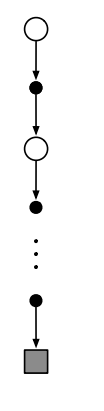
\includegraphics[width=0.1\textwidth]{/chapter5_1}
	\caption{Monte carlo backup diagram for one episode}
	\label{fig:monte carlo backup}
\end{figure}

\item Importantly, monte carlo methods do not bootstrap in the same way DP methods do. They take the reward at the end of an episode, rather than estimated reward based on the value of the next state.
\item Because of the lack of bootstrapping, this expense of estimating the value of one state is independent of the number of states, unlike DP. A significant advantage, in addition to the other advantages of being able to learn from experience without a model or from simulated experience. 
\end{itemize}

\subsection{Monte Carlo Estimation of Action Values}
\begin{itemize}
\item With a model we only need to estimate the state value function \(v\) as, paired with our model, we can evaluate the rewards and next states for each of our actions and pick the best one.
\item With model free methods we need to estimate the state-action value function \(q\) as we must explicitly estimate the value of each action in order for the values to be useful in suggesting a policy. (If we only have the values of states, and don't know how states are linked through a model, then selecting the optimal action is impossible)
\item One serious complication arises when we do not visit every state, as can be the case if our policy is deterministic. If we do not visit states then we do not observe returns from these states and cannot estimate their value. We therefore need to \textit{maintain exploration} of the state space. One way of doing so is stochastically selected a state-action pair to start an episode, giving every state-action pair a non-zero probability of being selected. In this case, we are said to be utilising \textit{\textbf{exploring starts}}.
\item Exploring starts falls down when learning from real experience because we cannot guarantee that we start in a new state-action pair in the real world. 
\item An alternative approach is to use stochastic policies that have non-zero probability of selecting each state-action pair.
\end{itemize}


\subsection{Monte Carlo Control}
\begin{itemize}
\item Much like we did with value iteration, we do not need to fully evaluate the value function for a given policy in monte carlo control. Instead we can merely \textit{move} the value toward the correct value and then switch to policy improvement thereafter. It is natural to do this episodically i.e. evaluate the policy using one episode of experience, then act greedily w.r.t the previous value function to improve the policy in the next episode.
\item If we use a deterministic policy for control, we must use exploring starts to ensure sufficient exploration. This creates the \textit{Monte Carlo ES} algorithm.
\end{itemize}

\subsection{Monte Carlo Control without Exploring Starts}
\begin{itemize}
\item To avoid having to use exploring starts we can use either \textit{on-policy} or \textit{off-policy} methods. The only way to ensure we visit everything is to visit them directly.
\item On-policy methods attempt to improve or evaluate or improve the policy that is making decisions.
\item On-policy control methods are generally \textit{soft} meaning that they assign non-zero probability to each possible action in a state e.g. e-greedy policies.
\item We take actions in the environment using e-greedy policy, after each episode we back propagate the rewards to obtain the value function for our e-greedy policy. Then we perform policy improvement by updating our policy to take the \textbf{new} greedy reward in each state. Note: based on our new value function, the new greedy action may have changed in some states. Then we perform policy evaluation using our new e-greedy policy and repeat (as per generalised policy iteration).
\item The idea of on-policy Monte Carlo control is still that of GPI. We use first visit MC methods to estimate the action-value function i.e. to do policy evaluation, but we cannot then make improve our policy merely by acting greedily w.r.t our value function because that would prevent further exploration of non-greedy actions. We must maintain exploration and so improve the $\epsilon$-greedy version of our policy. That is to say, when we find the greedy action (the action that maximises our reward for our given value function) we assign it probability $1 - \epsilon + \frac{\epsilon}{\mathcal{A}(S_t)}$ of being selected so that the policy remains stochastic.
\item Note: doing the above will only find us the best policy amongst the $\epsilon$-soft policies, which may not be the optimal policy for the environment, but it does allow us to remove the need for exploratory starts.
\end{itemize}

\subsection{Off-policy Prediction via Importance Sampling}
We face a dilemma when learning control: we want to find the optimal policy, but we can only find the optimal policy by acting suboptimally to explore sufficient actions. What we saw with on-policy learning was a compromise - it learns action values not for the optimal policy but for a near-optimal policy that still explores. An alternative is off-policy control where we have two policies: one used to generate the data (behaviour policy) and one that is learned for control (target policy). This is called \textit{off policy learning}.

\begin{itemize}
\item Off-policy learning methods are powerful and more general than on-policy methods (on-policy methods being a special case of off-policy where target and behaviour policies are the same). They can be used to learn from data generated by a conventional non-learning controller or from a human expert.
\item If we consider an example of finding target policy $\pi$ using episodes collected through a behaviour policy $b$, we require that every action in $\pi$ must also be taken, at least occasionally, by $b$ i.e. $\pi(a|s) > 0$ implies $b(a|s) > 0$. This is called the assumption of \textit{\textbf{coverage}}. 
\item Almost all off-policy methods utilize \textit{importance sampling}, a general technique for estimating expected values under one distribution given samples from another. Given a starting state $S_t$, the probability of the subsequent state-action trajectory occuring under any policy $\pi$ is:

\begin{equation}
	\prod_{k=t}^{T-1} \pi(A_k|S_k)p(S_{k+1}|S_k, A_k)
\end{equation}

where $p$ is the state transition probability function. We can then obtain the relative probability of the trajectory under the target and behaviour policies (the importance sampling ratio) as:

\begin{equation}
p_{t:T-1} = \frac{\prod_{k=t}^{T-1} \pi(A_k|S_k)p(S_{k+1}|S_k, A_k)}{\prod_{k=t}^{T-1} b(A_k|S_k)p(S_{k+1}|S_k, A_k)} = \prod_{k=t}^{T-1} \frac{\pi(A_k|S_k)}{b(A_k|S_k)}
\end{equation}

We see here that the state transition probability function helpfully cancels.

\item We want to estimate the expected returns under the target policy but we only have returns from the behaviour policy. To address this we simply multiply expected returns from the behaviour policy by the importance sampling ratio to get the value function for our target policy.

\begin{equation}
\mathbb{E} \left[p_{t:T-1} G_t | S_t = s\right] = v_\pi(s)
\end{equation}

\item Note: importance sampling ratios are only non-zero for episodes where the target-policy has non-zero probability of acting \textit{exactly} like the behaviour policy $b$. So, if the behaviour policy takes 10 steps in an episode, each of these 10 steps have to have been \textit{possible} by the target policy, else $\pi(a|s) = 0$ and $\rho_{t:T-1} = 0$.

\end{itemize}

\subsection{Incremental Implementation}
We perform monte carlo policy evaluation (prediction) incrementally in the same way as was done in Chapter 2 for the bandit problem. Generally incremental implementation follows this formula:

\begin{equation}
New Estimate \leftarrow Old Estimate + Step Size \left[Observation - Old Estimate \right]
\end{equation}

With on-policy monte carlo methods, this update is performed exactly after each episode for each visit to a state given the observed rewards, with off-policy methods the update is slightly more complex. With ordinary importance sampling, the step size is $1/n$ where $n$ is the number of visits to that state, and so acts as an average of the scaled returns. For weighted importance sampling, we have to form a weighted average of the returns which requires us to keep track of the weights. If the weight takes the form $W_i = \rho_{t:T(t)-1}$ then our update rule is:

\begin{equation} \label{incremental V}
V_{n+1} = V_n + \frac{W_n}{C_n}\left[G_n - V_n\right]
\end{equation}
where,
\begin{equation}
C_{n+1} = C_n + W_{n+1}
\end{equation}
with $C_0 = 0$. This allows us to keep tracking of the corrected weighted average term for each update as they are made. Note here that the weighted average gives more weight to updates based on common trajectories from $b$ in $\pi$ that we have some more often.

\subsection{Off-policy Monte Carlo Control}
Using incremental implementation (updates to the value function) and importance sampling we can now discuss \textit{off-policy monte carlo control}–the algorithm for obtaining optimal policy $\pi_*$ by using rewards obtained through behaviour policy $b$. This works in much the same way as in previous sections; $b$ must be $\epsilon$-soft to ensure the entire state space is explored in the limit; updates are only made to our estimate for $q_\pi$, $Q$, if the sequence of states an actions produced by $b$ could have been produced by $\pi$. This algorithm is also based on GPI: we update our estimate of $Q$ using Equation \ref*{incremental V}, then update $\pi$ by acting greedily w.r.t to our value function. If this policy improvement changes our policy such that the trajectory we are in from $b$ no longer obeys our policy, then we exit the episode and start again. The full algorithm is shown in \ref*{fig:Off-policy monte carlo control}.

\begin{figure}[h!]
	\centering
	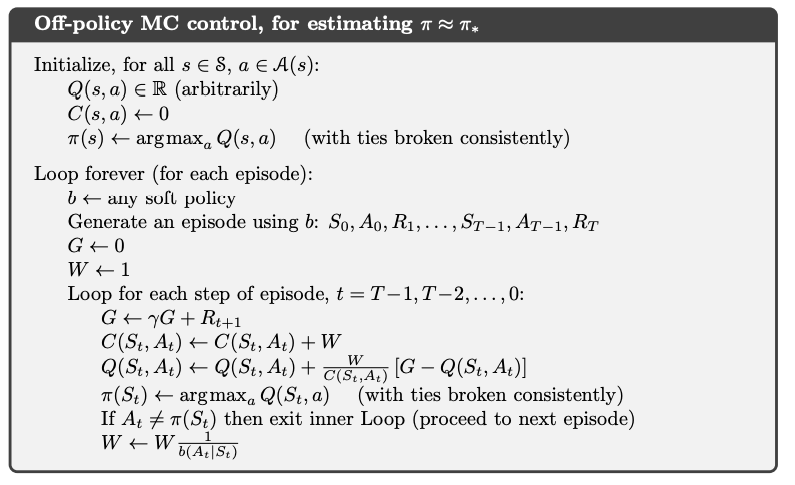
\includegraphics[width=0.5\textwidth]{/chapter5_3}
	\caption{Off-policy monte carlo control}
	\label{fig:Off-policy monte carlo control}
\end{figure}

\subsection{Key Takeaways}
\begin{itemize}
\item In the absence of a model of the environment, monte carlo methods allow us to evaluate and improve our value function based on \textit{experience}
\item We roll-out trajectories to terminal states, and back-propagate the rewards to the states visited en-route in several ways
\item Monte carlo methods use GPI (see chapter 4) in much the same way dynamic programming does. We evaluate our policy, then improve by acting greedily w.r.t our new value function until we converge on the optimal value function and policy.
\item Differences with dynamic programming methods: 1) They do not require a model of the environment as they learn directly from experience, and 2) They do not bootstrap i.e. the value function estimates are an average of all real returns accumulated after visiting the state.
\item Maintaining sufficient exploration is crucial with monte carlo methods; if our policy is deterministic we will likely not explore the full states space during our roll-outs. To deal with this we have several options: 1) Start every episode randomly with uniform probability such that we make sure we start at each possible state–called \textit{exploring starts}, unrealistic in the real world as we can't make a robot restart from all possible states. Or 2) Use $\epsilon$-soft policies that have a non-zero probability of selecting all possible states. The downside of doing this is that we will converge on the optimal $\epsilon$-soft, which is not necessarily the optimal policy for the environment, because it needs to learn how account for its own randomness. This is the price we pay for exploration.
\item Monte carlo methods can either be \textit{on-policy} or \textit{off-policy}.
\item On-policy methods use the same policy to collect data as is evaluated and improved. This suffers the downsides outlined above.
\item Off-policy methods have two policies, one that collects the data called the \textit{behaviour policy} $b$ and the other which we look to improve called the target policy $\pi$. We find trajectories from the behaviour policy that line up with our target policy, that is to say, that could have been produced by our target policy. This process only works if the behaviour policy has non-zero probability of selecting each of the actions in the target policy, aka \textit{coverage} of the target policy. The agent explores, but learns a deterministic optimal policy offline that may be unrelated to the behaviour policy used to collect the experience.
\item Based on rewards observed by running the behaviour policy, we update our value function using \textit{importance sampling}, which measures, if effect, how likely the observed behaviour would have been given our target policy. For example, the target policy may take 1 of 4 actions with equal probability in each state. If we observe two timesteps from our beaviour policy, then our probability of selecting the actions taken by the behaviour policy would be $0.25 x 0.25$. 
\item We weight each return using the x\textit{importance sampling ratio}, a measure of how likely we were to produce the roll-out using the target policy compared to how likely we were to produce the roll-out using the behaviour policy. 
\item Importance sampling can be \textit{ordinary} i.e. an average of the returns observed from a state or \textit{weighted} where trajectories viewed more often, or with a higher importance sampling ratio give the value update more weight.

\end{itemize}
\section{Temporal-Difference Learning}

TD learning is novel to RL. It is a hybrid that lies between monte carlo and dynamic programming methods. As with those, TD learning uses GPI; control (policy improvement) works in much the same way, it is in the prediction of the value function (policy evaluation) where the distinctions lie.

\subsection{TD Prediction}
Monte carlo methods wait until the end of the episode before back-propagating the return to the states visited en-route. The simplest TD method (TD(0)) does not wait until the end of the episode, in fact, it updates its estimate of the value function $V(s)$ based on the instantaneous reward as follows:
\begin{equation} \label{eq: td}
V(S_t) \leftarrow V(S_t) + \alpha \left[R_{t+1} + \gamma V(S_{t+1}) - V(S_t)\right]
\end{equation}

Note here, that TD(0) \textit{bootstraps} in much the same way DP methods do i.e. it bases it's estimate of $V(s)$ on the value of the next state $V(s')$. TD methods therefore take both sampling from monte carlo, and bootstrapping from DP. The TD(0) backup diagram is shown in Figure \ref{fig:td(0)}.

\begin{figure}[h!]
	\centering
	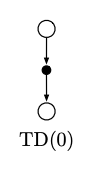
\includegraphics[width=0.2\textwidth]{/chapter6_1}
	\caption{Backup diagram for TD(0)}
	\label{fig:td(0)}
\end{figure}

The quantity in the brackets of equation \ref{eq: td} is known as the \textit{TD error}. Formally this is expressed as:
\begin{equation}
\delta_t = R_{t+1} + \gamma V(S_{t+1}) - V(S_t)
\end{equation}

\begin{figure}[h!]
	\centering
	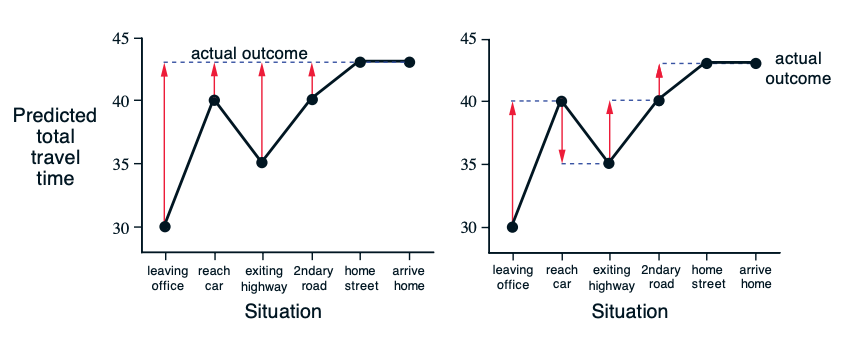
\includegraphics[width=\textwidth]{/chapter6_2}
	\caption{Monte carlo updates (left) and TD-updates (right) to the value function associated with a daily commute}
	\label{fig:td vs. mc}
\end{figure}

In Figure \ref{fig:td vs. mc} we see the differences between monte carlo and TD updates to the value function. In the case of monte carlo, we would need to wait until we arrived home before we could update our predictions for journey length. With TD learning, we can adjust these estimates on the fly based on the error in our predictions en-route. We see here that the adjustment we make changes at each timestep depending on the difference between predictions, that is to say, the update is proportional to the \textit{temporal differences} between our predictions across timesteps.

\subsection{Advantages of TD Prediction Methods}
\begin{itemize}
\item TD methods generally converge faster than MC methods, although this has not been formally proven.
\item TD methods do converge on the value function with a sufficiently small step size parameter, or with a decreasing stepsize.
\item They are extremely useful for continuing tasks that cannot be broken down in episodes as required by MC methods.
\end{itemize}

\subsection{Optimality of TD(0)}
If we only have a finite number of episodes or training data to learn from we can update our value function in \textit{batches}. We repeatedly play the same data, and update our value function by the sum of each of the increments for each state at the end of the batch.

TD batching and Monte Carlo batching converge often on two different estimates of the value function. The monte carlo batch estimate can only judge based on observed rewards from a state, but TD batching can make estimates based on later states using bootstrapping. Example 6.4 (\textit{You are the predictor}) on pg 127 explains this excellently. The monte carlo estimate will converge on the correct estimate of the value function produced by the training data, but TD methods will generalise better to future rewards because they preserve the transition from state-to-state in the TD update, and thus bootstrap better from values of other states.

In general batch MC methods always minimise the mean squared error or the training set whereas TD(0) finds the estimates that would be exactly correct for the maximum-likelihood model of the Markov process. This is called the \textit{certainty equivalence estimate} because it is equivalent to assuming that the estimate of the underlying process was known with certainty rather than being approximated.

\subsection{Sarsa: On-policy TD Control}
We'll now look at using TD prediction methods for control. We'll follow, as before, the framework of Generalised Policy Iteration (GPI), only this time using TD methods for predicting the value function.
For on-policy control, we wish to learn the state-action value function for our policy $q_\pi(s,a)$ and all states $s$ and actions $a$. We amend the TD update formula provided in Equation \ref{eq: td} to account for state-action values:
\begin{equation}
Q(S_t, A_t) \leftarrow Q(S_t, A_t) + \alpha \left[R_{t+1} + \gamma Q(S_{t+1}, A_{t+1}) - Q(S_t, A_t) \right]
\end{equation}

This produces a quintuple of events: $(S_t, A_t, R_{t+1}, S_{}t+1}, A_{t+1})$ giving rise to the name SARSA. As with other on-policy control algorithms, we update our policy to be greedy w.r.t our ever-changing value function. 















\section{$n$-step Bootstrapping}
In the previous chapter we discussed one-step TD prediction, and in the chapter previous to that we discussed monte carlo methods where predictions are made based on returns at the end of the episode. In this chapter we will discuss an approach between these two, where predictions are made after $n$-steps in the future. Doing so is often more effective than either of the two previously presented approaches. 

\subsection{$n$-step TD Prediction}
The spectrum of $n$-step TD methods is summarised by Figure \ref{fig: n-step methods}. Recall from the previous chapter that our one-step return used for TD(0) was:
\begin{equation}
	G_{t:t+1} = R_{t+1} + \gamma V_t(S_{t+1})
\end{equation}
we can generalise this to the $n$-step case as follows:
\begin{equation}
	G_{t:t+n} = R_{t+1} + \gamma R_{t+2} + \cdots + \gamma^{n-1}R_{t+n} + \gamma^nV_{t+n-1}(S_{t+n})
\end{equation}
for all $n, t$ such that $n \geq 1$ and $0 \leq t \leq T - n$. All $n$-step returns can be considered approximations to the full return, truncated after $n$ steps and then corrected for the remaining missing terms by $V_{t+n-1}(S_{t+n})$. If the n-step return extends to or beyond termination then all the missing terms are taken as zero.

\begin{figure}[h!]
	\centering
	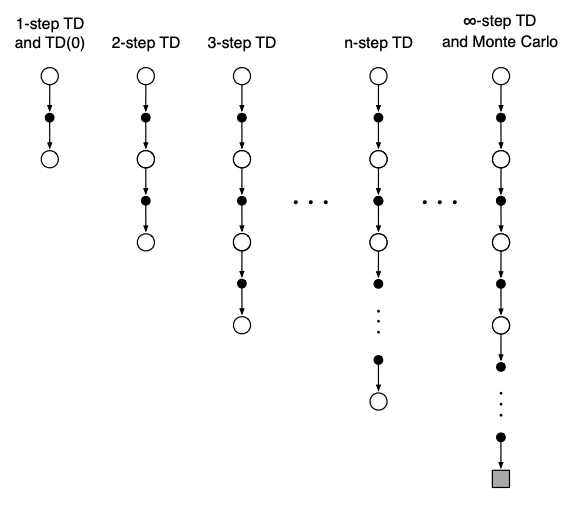
\includegraphics[width=0.7\textwidth]{/chapter7_1}
	\caption{Backup diagram for TD(0)}
	\label{fig: n-step methods}
\end{figure}\label{key}

The $n$-step return uses the value function $V_{t+n-1}$ to correct for missing rewards beyond $R_{t+n}$. An important property of $n$-step returns is that their expectation is guaranteed to be a better estimate of $v_\pi$ that $V_{t+n-1}$ in a worst-state sense i.e.:
\begin{equation}
\max_{s}|\mathbb{E}_\pi \left[G_{t:t+n} | S_t = s\right] - v_\pi(s)| \leq \gamma^n \max_{s} |V_{t+n-1}(s) - v_\pi(s)|
\end{equation}

This is called the error reduction property of $n$-step returns. Because of this, one can show formally that all $n$-step TD methods converge to t he correct predictions under appropriate conditions.

\subsection{$n$-step Sarsa}
We can extend $n$-step value function prediction to a control algorithm by incorporating the ideas of the Sarsa. Now, instead of making value function updates based on rewards received to the $t+n^{th}$ state, we select update our state-action value function $Q$ by making updates up to the $t+n^{th}$ state-action pair. The family of $n$-step Sarsa backup diagrams is shown in Figure \ref{fig: n-step sarsa methods}. The $n$-step Sarsa update is:
\begin{equation} \label{eq: n-step sarsa}
Q_{t+n}(S_t, A_t) = Q_{t+n-1}(S_t, A_t) + \alpha \left[G_{t:t+n} - Q_{t+n-1}(S_t, A_t)\right]
\end{equation}

\begin{figure}[h!]
	\centering
	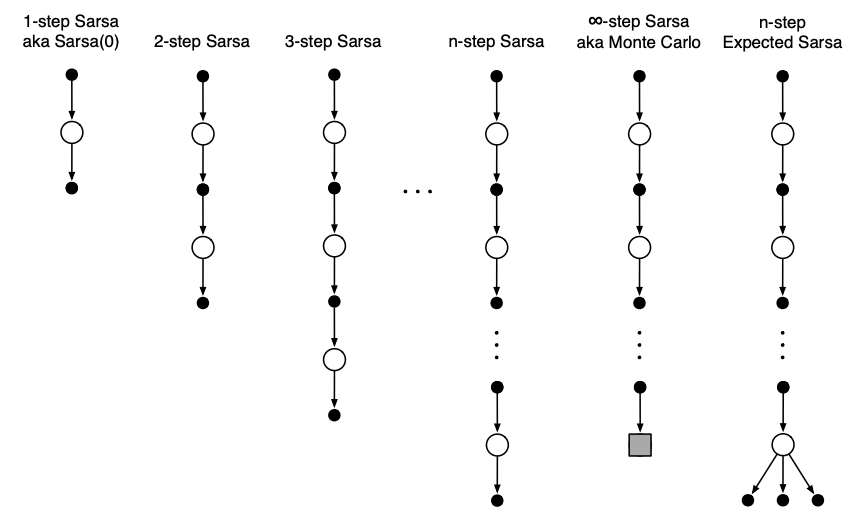
\includegraphics[width=0.7\textwidth]{/chapter7_2}
	\caption{Backup diagrams for family of $n$-step Sarsa algorithms}
	\label{fig: n-step sarsa methods}
\end{figure}

An example of why $n$-step sarsa speeds up policy learning is given in Figure \ref{fig: n-step sarsa speed up}
\begin{figure}
	\centering
	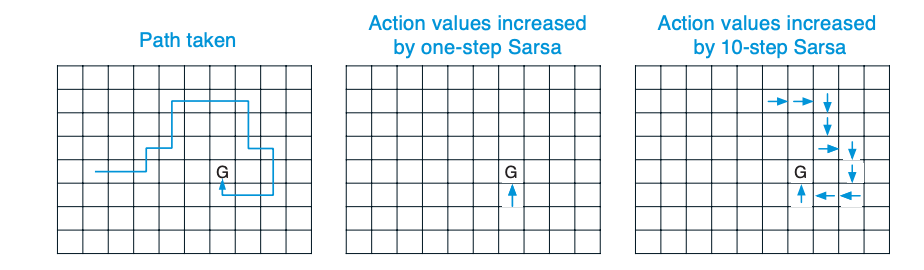
\includegraphics[width=0.8\textwidth]{/chapter7_3}
	\caption{Gridworld example of the speedup of policy learning due to the use of n-step methods. The first panel shows the path taken by an agent in a single episode, ending at a location of high reward, marked by the G. In this example the values were all initially 0, and all rewards were zero except for a positive reward at G. The arrows in the other two panels show which action values were strengthened as a result of this path by one-step and n-step Sarsa methods. The one-step method strengthens only the last action of the sequence of actions that led to the high reward, whereas the n-step method strengthens the last n actions of the sequence, so that much more is learned from the one episode.}
	\label{fig: n-step sarsa speed up}
\end{figure}

Expected Sarsa remains an important version of Sarsa because of the variance-reducing expectation. The algorithm is described as in equation \ref{eq: n-step sarsa}, but this time the expected return includes the expected value of the final value function, i.e.:
\begin{equation}
G_{t:t+n} = R_{t+1} + \cdots + \gamma^{n-1}R_{t+n} + \gamma^n \bar{V}_{t+n-1}(S_{t+n})
\end{equation}
where $\bar{V}_{t+n-1}(s)$ is the \textit{expected approximate value} of state $s$, using the estimated action values at time $t$, under the target policy:
\begin{equation}
\bar{V}_{t}(s) \doteq \sum_{a} \pi(a|s) Q_t(s,a), \; \; \text{for all} \; s \in \mathcal{S}
\end{equation}

Expected approximate values are used in developing many of the action-value method discussed hereafter. 

\subsection{$n$-step Off-policy Learning}
We can extend $n$-step learning to the off-policy case where we have a behaviour policy $b$ that creates the data and a target policy $\pi$ that we wish to update. As previously discussed, when we make updates in this way, we must weight the updates using the importance sampling ratio - equation \ref{eq: importance sampling ratio}. We can create a generalised form of the $n$-step algorithm, that works for both on-policy and off-policy cases:
\begin{equation}
Q_{t+n}(S_t, A_t) = Q_{t+n-1}(S_t, A_t) + \alpha \rho_{t+1:t+n} \left[G_{t:t+n} - Q_{t+n-1}(S_t, A_t)\right]
\end{equation}

\subsection{Per-decision Methods with Control Variates}
The off-policy methods described above may not learn as efficiently as they could. If we consider the case where the behaviour policy does not match the target policy for one of the $n$ steps used in the update, the update will go to 0 and the value function estimate will not change. Instead we can use a more sophisticated approach, that has a different definiton of the $n$-step horizon:
\begin{equation} \label{eq: off policy n step}
G_{t:h} \doteq \rho_t (R_{t+1} + \gamma G_{t+1:h}) + (1 - \rho_t)V_{h-1}(S_t)
\end{equation}

In this approach, if $\rho_t$ is zero, then instead of the target being zero and causing the estimate to shrink, the target is the same as the estimate and causes no change. Because the expected value of $\rho_t$ is 1, the expected value of the second term in equation \ref{eq: off policy n step}, called the \textit{control variate} has expected value of 0, and so does not change the update in expectation.

\subsection{Off-policy Learning Without Importance Sampling: The $n$-step Tree Backup Algorithm}
Here we will discuss off-policy learning without the need for importance sampling, conceptualised by the $n$-step Tree Backup Algorithm–Figure \ref{fig: tree-backup update}. In this tree backup update, the target now includes all rewards \textit{plus} the estimated values of the dangling action nodes hanging off the sides, at all levels. It is an update from the \textit{entire tree} of estimated action values. For each node in the tree backup diagram, we the estimated values of the non-selected actions are weighted  by their probability of being selected under our policy $\pi(A_t|S_t)$. The value of the selected action does not contribute at all at this stage, instead its probability of being selected weights the instantaneous reward of the next state \textit{and} each of the non-selected actions at the next state, which too are weighted by their probabilities of occurring as described previously. Formally, the one-step return is as follows:
\begin{equation}
G_{t:t+1} \doteq R_{t+1} + \gamma \sum_{a} \pi(a | S_{t+1}) Q_t(S_{t+1}, a)
\end{equation}

the two-step backup return (for $t < T - 1$) is described recursively as:
\begin{equation}
G_{t:t+2} \doteq R_{t+1} + \gamma \sum_{a \neq A_{t+1}} \pi(a | S_{t+1}) Q_t(S_{t+1}, a) + \gamma \pi(A_{t+1} | S_{t+1})G_{t+1:t+2}
\end{equation}

in the general case this becomes:
\begin{equation}
G_{t:t+n} \doteq R_{t+1} + \gamma \sum_{a \neq A_{t+1}} \pi(a | S_{t+1}) Q_{t+n-1}(S_{t+1}, a) + \gamma \pi(A_{t+1} | S_{t+1})G_{t+1:t+n}
\end{equation}

These returns are then used in the normal action-value update for $n$-step sarsa, as described by equation \ref{eq: n-step sarsa}.

\begin{figure}
	\centering
	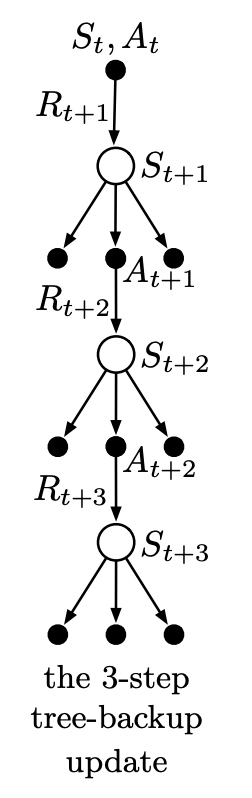
\includegraphics[width=0.25\textwidth]{/chapter7_4}
	\caption{The 3-step tree-backup update}
	\label{fig: tree-backup update}
\end{figure}

\subsection{A Unifying Algorithm: $n$-step Q($\sigma$)}
We'd like an algorithm that generalises the differences between n-step sarsa, as discussed at the beginning of this chapter, and n-step tree backup as discussed at the end of this chapter. To do so, we create a new algorithm parameter $\sigma \in [0,1)]$ that acts as a linear interpolator between the two extreme cases. This allows us to do a full, expected tree back-up in some cases, and a straight sarsa update on others, or work in the continuous region between. The family of algorithms explored in this chapter are summarised in figure \ref{fig: all chap 7 backup diagrams}:

\begin{figure}
	\centering
	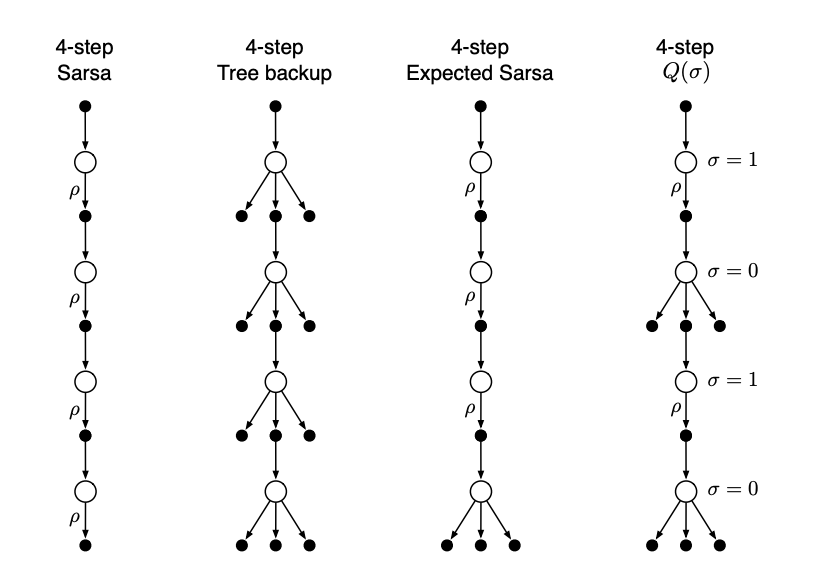
\includegraphics[width=0.75\textwidth]{/chapter7_5}
	\caption{The backup diagrams of the three kinds of n-step action-value updates considered so far in this chapter (4-step case) plus the backup diagram of a fourth kind of update that unifies them all. The label ‘$\rho$’ indicates half transitions on which importance sampling is required in the off-policy case. The fourth kind of update unifies all the others by choosing o a state-by-state basis whether to sample ($\sigma_t$ = 1) or not ($\sigma_t$= 0).}
	\label{fig: all chap 7 backup diagrams}
\end{figure}

\subsection{Key Takeaways}
\begin{itemize}
\item $n$-step TD methods lie between one-step TD methods as described in the previous chapter and full Monte Carlo backups as described in the chapter two previous. They typically perform better than either of these extremes.
\item $n$-step sarsa is an on-policy algorithm that updates state-action values based on rewards obtaining $n$ timesteps into the future following our policy $\pi$.
\item $n$-step off policy learning corrects for the failures of on-policy learning by weighting updates by the importance sampling ratio $\rho_t$ as discussed in chapter 6.
\item Variance in the off-policy $n$-step updates can be reduced using \textit{per-decision methods with control variates} that stop the value update being 0 if the behaviour policy $b$ does not match the target policy $\pi$ for any of the $n$ timesteps.
\item Finally, these methods are all more complex (expensive), and require additional memory, than one-step TD methods discussed previous.
\item We can do without importance sampling if our update is based on an expectation over each of the state-action values visited along our $n$-step trajectory. This is called the \textit{$n$-step tree backup algorithm}.
\item The continuum between all of these discussed methods can be traversed using the $n$-step Q($\sigma$) algorithm that characterised at which time steps we take full expectations and which we use only the sarsa update.
\end{itemize}
\section{Planning and Learning with Tabular Methods}
RL methods can be described as either \textit{model-based} or \textit{model-free}. Model-based methods rely on \textit{planning} as their primary component, while model-free methods rely on \textit{learning}. Despite their differences, both still use value functions and both make backups to state values based on future returns or estimates. This chapter will provide a unifying framework for model-free and model-based RL methods.

\subsection{Models and Planning}
\begin{itemize}
	\item Models are anything the agent can use to predict the outcome of its actions.
	\item Models can be either \textit{distribution models} or \textit{sample models}. The former is a probability distribution over all possible next states whereas the latter produces one of the possible next states sampled from the probability distribution.
	\item Distribution models are stronger than sample models because they can always be used to create samples, but sample models are easier to create in practice.
	\item Models are used to \textit{simulate} the environment thus producing \textit{simulated experience}. Distribution models could produce every possible episode, weighted by their probability of occurring, whereas sample models can only produce one episode.
	\item The word \textit{planning} refers to any computational process that takes a model as input and produces or improves a policy for interacting with the modelled environment.
	\item The common structure of updating our policy by utilising our model is given in Figure \ref{fig: updating policy using model}.
	\item We can use models in place of the real environment to perform model-free learning safely i.e. using simulated experience rather than real experience.
\end{itemize}

\begin{figure} [h!]
	\centering
	
\includegraphics[width=\textwidth]{/chapter8_1}
	\caption{The framework for updating our policy using our model of the environment}
	\label{fig: updating policy using model}
\end{figure}

\subsection{Dyna: Integrated Planning, Acting, and Learning}
Instead of planning all possible future states permutation, we may want to plan over a small number of future timesteps. When we do this we will likely want to update both our policy and model \textit{online}. The canonical algorithm for doing so is \textbf{Dyna-Q}. 
\begin{itemize}
\item Planning agents can use the experience they collect to do one of two things: 1) improve the model (also called \textit{model-learning}) and 2) improve the value function and policy (also called \textit{direct reinforcement learning (direct RL)}). These options are summarised in  \ref{fig: direct rl and model-learning}. Sometimes model-learning is called \textit{indirect RL} because improving our model, improves our policy by proxy.
\item Dyna-Q agents conduct direct RL, planning, model-learning and acting simultaneously. Planning and direct learning tend to use exactly the same machinery as each other e.g. $n$-step sarsa, and thus are closely linked. Figure \ref{fig: dyna} shows the generalised Dyna architecture.
\item Planning (in Dyna Q) is the process of running our Q updates (from Q-learning) using our model. We select random states and actions previously taken, find the reward and next state using our model and make the Q update. We do this $n$ times for each timestep taken in the real environment, where $n$ is a hyper parameter. For each unit of real experience collected, we are updated our value function $n$ simultaneously.
\end{itemize}

\begin{figure}
	\centering
	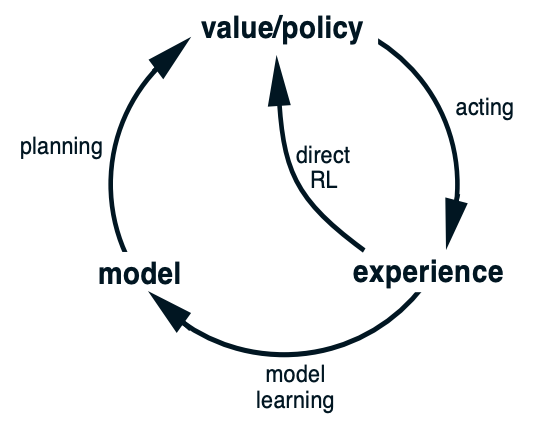
\includegraphics[width=0.5\textwidth]{/chapter8_2}
	\caption{Direct RL and model-learning, either achieved using data collected from experience}
	\label{fig: direct rl and model-learning}
\end{figure}

\begin{figure}
	\centering
	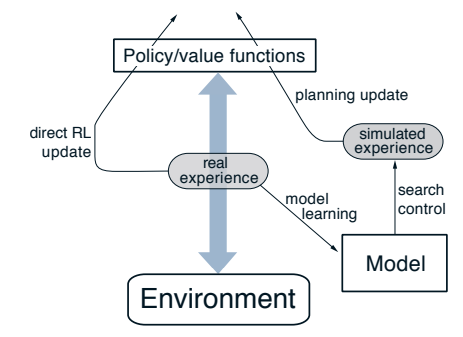
\includegraphics[width=0.75\textwidth]{/chapter8_3}
	\caption{Generalised Dyna architecture}
	\label{fig: dyna}
\end{figure}

\subsection{When the Model is Wrong}
Often our model will be wrong. This can happen initially because the environment is stochastic and we haven't collected enough samples to evaluate this stochasticty accurately. Otherwise, it can happen because we've used function approximation (e.g. neural networks) to predict the model, which generally arrive with non-zero error. When the model is incorrect the planning process is likely to compute a suboptimal policy. Often the suboptimal policy quickly leads to the discovery and correction of modelling error, as when the agent takes actions prescribed by the planned policy in the real environment, it quickly finds the expected rewards are incorrect or do not exist. 

Issues arise when the environment changes to become \textit{better} or more favourable at some stage during learning. In these cases the optimal policy/route to goal remains unchanged, but there is an even better policy available that the agent may never access because it has no reason to doubt its previously learned optimal policy. To address this, another algorithm is proposed called Dyna-Q+. Here, the agent keeps track of the number of timesteps elapsed $\tau$ since a state-action pair had been selected, and, if sufficient time has elapsed, it is presumed that the dynamics of the environment from that state have changed. The modelled rewards for each state-action pair now take the form $r + k\sqrt{\tau}$ for some small $k$.

\subsection{Prioritized Sweeping}
Until now, updates made to the value function during planning have been made arbitrarily, that is to say, state-actions have been sampled uniformly from past experience regardless of how likely we are to visit those state-actions. It would be more useful to prioritize updates to the value function that would be most effected by the reward we have recently received. This general idea is termed \textit{backward focusing} of planning computations. If we prioritize the updates according to a measure of urgency and perform them in order of priority, we call this \textit{prioritized sweeping}. The prioritization queue is assesmbled based on the expected update to a state-value pair from a new reward. We then loop through this queue, and for each state-value pair, find the state-value pairs we would predict lead to it, and calculated \textit{their} expected update and add them to the queue. The additions to the queue are only made if the expected update is larger than some value $\theta$. In this way, we only plan based on state-value pairs whose value updates are non-trivial. This technique is regularly 5-10 times faster than Dyna-Q.

\subsection{Expected vs. Sample Updates}
This book began by discussing dynamic programming; a way of conducting policy evaluation and improvement given a distribution model of the environment. Then we discussed sampling methods like: monte carlo, temporal-difference methods and n-step bootstrapping to estimate value functions in the absence of a model. Implicit here, was the idea that a distribution model than can be used to compute expectations is better than sampling which often leads to higher variance through sampling error. But is this true? To properly assess the relative merits of expected and sample updates for planning we must control for their different computational requirements.

In practice, the computation required by update operations is usually dominated by the number of state-action pairs at which $Q$ is evaluated. For a particular starting pair, $s, a$, let $b$ be the \textit{branching factor} (i.e. the number of possible next states, $s'$ for which $\hat{p}(s|s,a)>0$. Then an expected update of this pair requires roughly $b$ times as much computation as a sample update. If we have sufficient time to complete an expected update, it is usually better than that of $b$ sample updates because of the absence of sampling error. But if there is insufficient time, sampling is always better because some update is better than no update. The key question is therefore: given a unit of computational power, is it better to perform one expected update, or $b$ sample updates? An answer to this question is provide in Figure \ref{fig: samples vs expectations}. For large values of $b$ sampling has huge efficiency gains over expected updates. In reality this effect would be more pronounced as the values of the successor states would be estimates that are themselves updated. By causing estimates to be more accurate sooner, sample updates will have a second advantage in that the values backed up from the successor states will be more accurate.

\begin{figure}
	\centering
	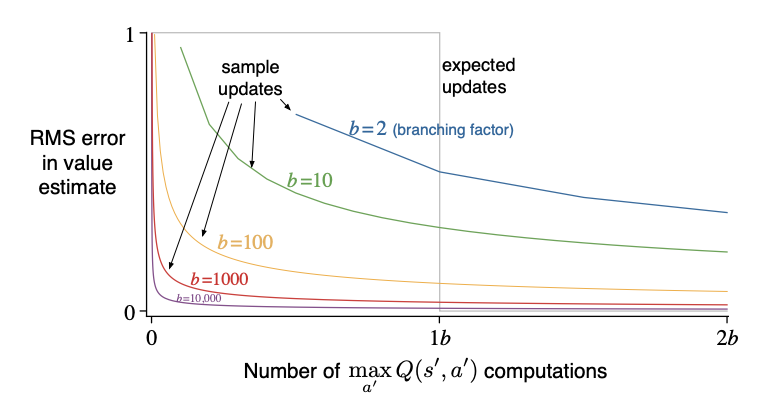
\includegraphics[width=\textwidth]{/chapter8_4}
	\caption{Comparison of efficiency of expected and sample updates}
	\label{fig: samples vs expectations}
\end{figure}

\subsection{Trajectory Sampling}
One could update every state-action pair, or state value, by performing full sweeps of the state space using dynamic programming. As discussed on several occasions this is computationally inefficient, given many of the states may have small probability of occurring. Instead we could sample from state-action space according to some distribution; uniformly in the case of Dyna Q, or according to an on-policy distribution that we observed following the current policy. We can do so by interacting with the model, simulating explicit individual trajectories and updating state or state-action pairs encountered along the way. We call this \textit{trajectory sampling}.

A question arises around whether on-policy updates, that follow the model's transition distribution, are better than updates made with uniform probability across the state-space. It seems for problems with large state-spaces, and small branching factors, it is advantageous to use on-policy distribution sampling. In the long run, however, focusing on the on-policy distribution may hurt because our estimates for these values are already well defined and we are not seeing unusual parts of the state space.

\subsection{Real-time Dynamic Programming}
Real-time dynamic programming (RTDP) is an on-policy trajectory-sampling version of the value iteration algorithm of dynamic programming (DP). Because the algorithm follows the on-policy distribution, our value iteration updates are more efficient that normal DP because we implicitly ignore irrelevant states to our policy in our updates. RTDP is guaranteed to find a policy that is optimal on the relevant states without visiting every state infinitely often, or even without visiting some states at all, under certain conditions. These are:
\begin{itemize}
	\item The intial value of every goal state is zero
	\item There exists at least one policy that guarantees that a goal state will be reached with probability one from any start state.
	\item All rewards for transitions from non-goal states are strictly negative, and
	\item All the initial values are equal to, or greater than, their optimal values (which can be satisfied by setting initial values to 0.)
\end{itemize}

Tasks with these properties are usually called \textit{stochastic optimal path problems}. RTDP can find optimal policies for these tasks with approximately 50\% of the computation required for traditional sweep-based value iteration i.e. dynamic programming.

\subsection{Planning at Decision Time}
The techniques discussed thus far have involved planning in between action-selection, we call this \textit{background planning}. Another way to do planning is at the time of action-selection i.e. to run trajectories or simulations in our model, and decide the optimal action to select based on the outcome of these trajectories. We call this \textit{decision-time planning}.

So we now have two ways of thinking about planning:
\begin{enumerate}
	\item Using simulated experience to gradually improve our policy or value function, or
	\item Using simulated experience to select an action for the current state
\end{enumerate}

Usually the results of this kind of planning are not used to update our value function or policy directly, and are generally discarded after action selection. This is fine for large state spaces, but if the state spaces are smaller than it can be expedient to keep these values and update our value function, such that we combine the two types of planning outlined above.

Decision-time planning is most useful in applications where fast response is not required, like chess. If low-latency actions are required, it's generally better to do planning in the background.

\subsection{Heuristic Search}
The canonical decision time planning method is \textit{heuristic search}. For each state encountered, heuristic search dedicates computational resource to searching a large tree of possible continuations, or state permutations thereafter. The search evaluates leaf nodes at the end of the search and backs up the values to the state-action nodes for the current states. The value maximising action from the current state is found and then selected. The values are usually discarded. This kind of planning is effective because it focuses only on pertinent next states and actions, and focuses resource on obtaining the next best one-step action. The backup diagram for heuristic search is shown in Figure \ref{fig: heuristic search}.

\begin{figure}
	\centering
	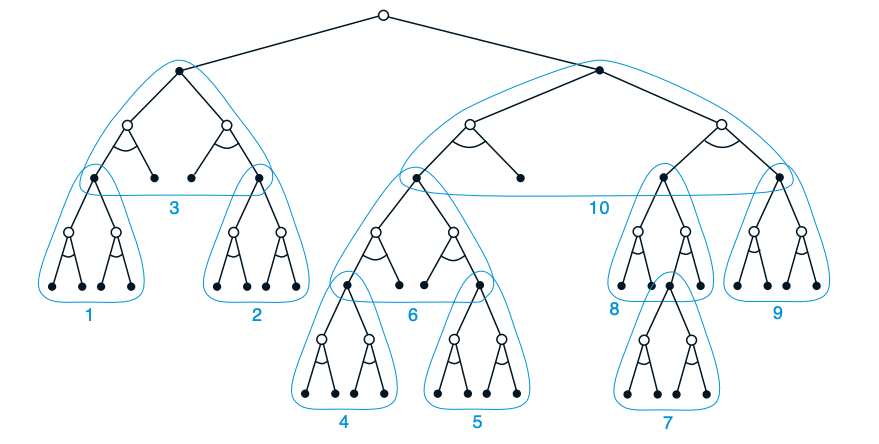
\includegraphics[width=\textwidth]{/chapter8_5}
	\caption{Heuristic search can be implemented as a sequence of one-step updates (shown here outlined in blue) backing up values from the leaf nodes toward the root. The ordering shown here is for a selective depth-first search.}
	\label{fig: heuristic search}
\end{figure}

\subsection{Rollout Algorithms}
Rollout algorithms apply Monte Carlo control to simulated trajectories that all begin at the current environment state. They estimate action values for a given policy by averaging the returns from many simulations in a model using the current policy. These algorithms, like heuristic search, make immediate use of these action value estimates then discard them, they do not attempt to estimate $q_*$ like monte carlo policy iteration as discussed in chapter 5. They take advantage of the mathematical properties of policy iteration discussed in chapter 4, that is, $\pi'$ > $\pi$ if both are identical except that $\pi'(s) = a \neq \pi(s)$ and $q_{\pi}(s,a) \geq v_\pi(s)$.

The limited factor with these types of algorithms is always computational resource, which itself is dependent on the size of the state-space. However there are ways around this, including pruning the rollouts to only involve the most probable next states, or to truncate simulated trajectories so they do not run to the end of the episode.

\subsection{Monte Carlo Tree Search}
Monte Carlo Tree Search (MCTS) is a rollout algorithm as described above, but with some modifications. Instead of rolling out trajectories randomly, MCTS first selects a small set of actions according to its \textit{tree policy}, then sometimes expands this selection to one or more actions, and then performs a full rollout to end of episode using a rollout policy. The value found upon termination of this trajectory is then backed up to the current state. This process is repeated for as long as time/computational constraints allow, then the agent selects an action usually based on which action produced best future estimated reward. MCTS is illustrated in Figure \ref{fig: MCTS}

\begin{figure}
	\centering
	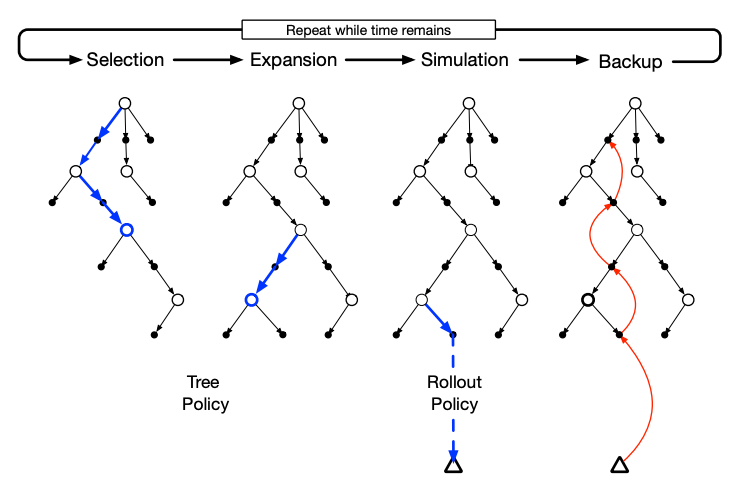
\includegraphics[width=\textwidth]{/chapter8_6}
	\caption{Monte Carlo Tree Search. When the environment changes to a new state, MCTS executes as many iterations as possible before an action needs to be selected, incrementally building a tree whose root node represents the current state. Each iteration consists of the four operations Selection, Expansion (though possibly skipped on some iterations), Simulation, and Backup, as explained in the text and illustrated by the bold arrows in the trees.}
	\label{fig: MCTS}
\end{figure}

\subsection{Key Takeaways}
\begin{itemize}
	\item Planning algorithms use models. These models can be either \textit{distribution models} that provide a probability distribution over next states (as required to compute expectations for dynamic programming), or can be \textit{sample models} that provide a sample of future states drawn from the underlying distribution that we are yet to access, or cannot access.
	\item Algorithms used for both learning and planning are often identical, the difference being that \textit{learning} involves updating our value function from real experience, whereas \textit{planning} involves updating our value function based on simulated experience from our model.
	\item Models can often be wrong, and the best way to ensure they stay up to date in continual maintain them through true experience. Sometimes we will obtain an optimal policy using a model that was once correct, but has since become redundant. We can attempt to keep an accurate model of our environment by taking actions in the environment that have not be attempted for some time to test the truth of our model. This technique is exhibited by Dyna Q+.
	\item Sample updates are often more efficient than expected updates for large state-spaces with large branching factors (a measure of the expected number of possible next states from an action).
	\item Trajectory sampling in our model can be used for planning. This can be useful when conducted on-policy, because we prioritise making updates to our value function that are particularly relevant to our policy.
	\item Planning can be conducted pre-action selection, to update our value function and inform future action-selection, or it can be done at the time of action-selection. The former is called \textit{background planning} and the latter is called \textit{decision time planning}.
	\item Examples of decision time planning include Heuristic Search (where value maximising actions are taken in a simulation of various next states, and backed up to the root node), Rollout Algorithms (where monte carlo rollouts are performed over many simulations of episodes and the value maximising action returned), or MCTS (a special case of rollout algorithms that effectively combines heuristic search over some small number of actions and then performs monte carlo rollouts thereafter).
	\item Decision time planning can be effective for tasks where low-latency action selection is not required. They are fundamentally limited by the time constraints on action-selection and on the available computational resource.
\end{itemize}

\subsection{Summary of Part 1}
\begin{figure}
	\centering
	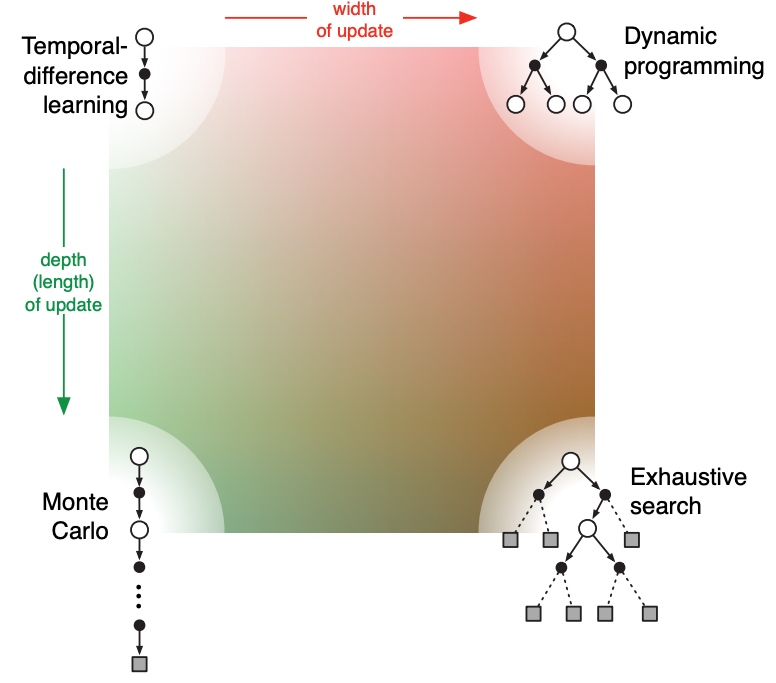
\includegraphics[width=\textwidth]{/chapter8_7}
	\caption{A slice through the space of reinforcement learning methods, highlighting the two of the most important dimensions explored in Part I of this book: the depth and width of the updates.}
	\label{fig: part1 summary}
\end{figure}


\section{On-policy Prediction with Approximation}
\subsection{Value-function Approximation}
Until now we have made updates to our value function in the tabular setting, we can, however, store our value function using some kind of function approximating technique with parameters $\textbf{w} \in \mathbb{R}^d$. Most function approximation techniques are examples of \textit{supervised learning} that require parameters $\textbf{w}$ to be found using training examples. In our case, we pass the function approximators our update to the value function online i.e. $s \rightarrowtail u$ where $u$ is the update ot the value function we'd like to make at state $s$.

\subsection{The Prediction Objective ($\bar{VE}$)}
Given we have far less parameters $\textbf{w}$ than states $s$ we cannot feasible approximate the value function perfectly. Indeed any updates we make the weights based on one state update will invariably lead to increased error at other states. We must therefore define which states we care about getting correct most, which we do with a state distribution $\mu(s) \geq 0, \sum_{s}\mu(s) = 1$. We can weight the error in prediction between our approximate value function $\hat{v}(s, \textbf{w})$ and the true value function $v_\pi(s)$ by this distribution to obtain our objective function, the \textit{mean square value error}:
\begin{equation}
\bar{VE}(\textbf{w}) \doteq \sum_{s \in \mathcal{S}} \mu(s)\left[v_\pi(s) - \hat{v}(s, \textbf{w})\right]^2
\end{equation}

Often $\mu(s)$ is chosen to be the fraction of time spent in $s$, called the \textit{on-policy distribution} in on-policy training.

\subsection{Stochastic-gradient and Semi-gradient Methods}
Our function approximator can be parametrised by a weight vector with a fixed number of real valued components, $\textbf{w} \doteq (w_1, w_2, \ldots, w_d)^T$. In \textit{stochastic gradient descent}, we update the weight vector at each timestep by moving it in the direction that minimises the error most quickly for the example shown:
\begin{align}
\textbf{w}_{t+1} &= \textbf{w}_t - \frac{1}{2}\alpha \nabla \left[v_\pi(S_t) - \hat{v}(S_t, \textbf{w}_t)\right]^2 \\
&= \textbf{w}_t + \alpha\left[v_\pi(S_t) - \hat{v}(S_t, \textbf{w}_t)\right] \nabla \hat{v}(S_t, \textbf{w}_t) 
\end{align}
where the second equation is obtained via the chain rule. Here, $\nabla f(\textbf{w})$ for any scalar expression $f(\textbf{w})$ that is a function of a vector (here \textbf{w}), denotes the column vector of partial derivatives of the expression with respect to the components of the vector:
\begin{equation}
	\nabla f(\textbf{w}) \doteq \left(\frac{\partial f(\textbf{w}) }{\partial w_1}, \frac{\partial f(\textbf{w}) }{\partial w_2}, \cdots, \frac{\partial f(\textbf{w}) }{\partial w_d}\right)^T.
\end{equation}

Often we will not know the \textit{true} value function that we are trying to approximate, and instead we will be using a bootstrapped value or some other approximation. In this case we replace $v_\pi(s)$ with $U_t$ which yields the following generalised SGD method for state-value prediction:

\begin{equation}
\textbf{w}_{t+1} =  \textbf{w}_t  + \alpha\left[U_t - \hat{v}(S_t, ))\right] \nabla \hat{v}(S_t, ) 
\end{equation}

If $U_t$ is an unbiased estimate, that is, if $\mathbb{E}[U_t | S_t =s] = v_\pi(s)$ then $\textbf{w}_t$ is guaranteed to converge to the local optimum. An example of an unbiased estimator is the monte carlo estimate for state $s_t$, unfortunately methods that use bootstrapping are biased in that their target is not independent of the the weights $ \textbf{w}_t $. We therefore call these methods \textit{semi-gradient methods}.

\subsection{Linear Methods}
Corresponding to every state $s$, there is a real-valued vector $\textbf{x}(s) \doteq (x_1(s), x_2(s), \ldots, x_d(s))^T$ with the same number of components as $\textbf{w}$. Linear methods approximate the state-value function by the inner product between $\textbf{w}$ and $\textbf{x}(s)$:
\begin{equation}
\hat{v}(s, \textbf{w}) \doteq \textbf{w}^T\textbf{x}(s) \doteq \sum_{i=1}^{d} w_ix_i(s)
\end{equation}

$\textbf{x}(s)$ is called a \textit{feature vector} representing state $s$. For linear methods, features are \textit{basis functions} because they form a linear basis for the set of approximate functions. For linear methods, the gradient of the approximate value function w.r.t \textbf{w} in this case is:
\begin{equation}
\hat{v}(s, \textbf{w})) = \textbf{x}(s)
\end{equation}
Thus the general SGD update reduces to a simple form:
\begin{equation}
\textbf{w}_{t+1} \doteq \textbf{w}_t + \alpha \left[U_t - \hat{v}(S_t, \textbf{w})\right]\textbf{x}(S_t)
\end{equation}

For the continuing case, the update at each time $t$ is:
\begin{align}
\textbf{w}_{t+1} &\doteq \textbf{w}_t + \alpha \left(R_{t+1} + \gamma \textbf{w}_t^T\textbf{x}_{t+1} - \textbf{w}_t^T \textbf{x}_t \right)\textbf{x}_t \\
&= \textbf{w}_t + \alpha \left(R_{t+1}\textbf{x}_{t} + \textbf{x}_{t}(\textbf{x}_{t} - \gamma \textbf{x}_{t+1}^T) \textbf{w}_t \right) \\
\end{align}

Once the system has reached steady state, for any given $\textbf{w}_t$, the expected next weight vector can be written as
\begin{equation}
\mathbb{E}[\textbf{w}_{t+1}|\textbf{w}_t] = \textbf{w}_t + \alpha(\textbf{b}-\textbf{Aw}_t)
\end{equation}
where
\begin{equation}
\textbf{b} \doteq \mathbb{E}[R_{t+1} \textbf{x}_t] \in \mathbb{R}^d \; \; \text{and} \; \; \textbf{A} \doteq \mathbb{E}\left[\textbf{x}_t(\textbf{x}_t - \gamma \textbf{x}_{t+1})^T\right] \in \mathbb{R}^{d \times d}
\end{equation}

It's therefore clear that the system must converge toward the weight vector $\textbf{w}_{TD}$ at which:
\begin{align}
\textbf{b-Aw}_{TD} &= 0 \\
b &= \textbf{Aw}_{TD} \\
\textbf{w}_{TD} &\doteq \textbf{A}^-1\textbf{b}
\end{align}

This quantity is called the \textit{TD fixed point}. The $n$-step semi-gradient TD algorithm for estimating $\hat{v} \approx v_\pi$ is given in Figure \ref{fig: n-step algo}.

\begin{figure}[h!]
	\centering
	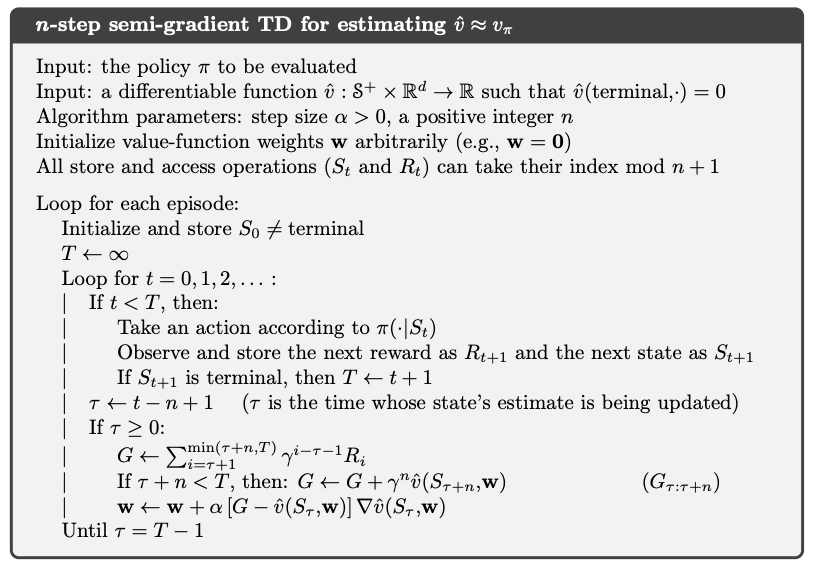
\includegraphics[width=\textwidth]{/chapter9_1}
	\caption{Algorithm: $n$-step semi-gradient TD for estimating $\hat{v} \approx v_\pi$}
	\label{fig: n-step algo}
\end{figure}

\subsection{Feature Construction for Linear Models}
Constructing features that are appropriate for the RL task is critical for providing the agent useful prior knowledge about the domain. In this section we will discuss different ways of constructing features.

\subsubsection{Polynomials}
We may want to design features with higher complexity than can be captured with linear methods. If we think of the example of parametrising a state $s$ by two dimensions $s_1 \in \mathbb{R}$ and $s_2 \in \mathbb{R}$, we could represent this state as $\textbf{x}(s) = (s_1, s_2)^T$. This, however, does not allow us to represent interactions between the two dimensions if they do indeed interact, and it would also mean that the value of our state would have to be 0 if both dimensions were zero. We can instead use a four-dimensional feature vector like: $\textbf{x}(s) = (1, s_1, s_2, s_1s_2)^T$. This allows us to capture any combination of these dimensions in polynomial space. The generalised form of polynomials is shown in Figure \ref{fig: poly}.

\begin{figure}[h!]
	\centering
	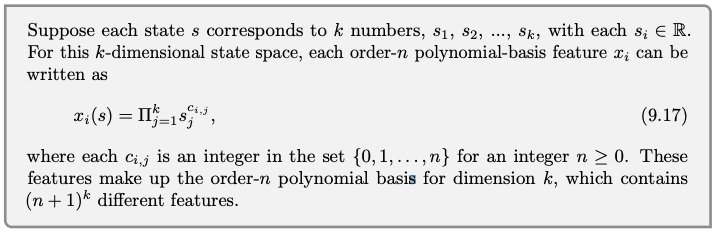
\includegraphics[width=\textwidth]{/chapter9_2}
	\caption{Generalised form of polynomial basis}
	\label{fig: poly}
\end{figure}

Note that $c_{i,j}$ here is a matrix with $i$ rows corresponding to $i$ features and $j$ columns corresponding to $j$ dimensions.

\subsubsection{Fourier Basis}
Fourier series express periodic functions as weighted sums of sine and cosine basis functions (as features) of different frequencies, with a function $f$ being periodic if $f(x) = f(x + \tau)$ for all $x$ and some period $\tau$. The one-dimensional, order-$n$ Fourier cosine basis consists of the $n+1$ features:
\begin{equation}
	x_i(s) = cos(i\pi s), \; \; \; s \in [0,1]
\end{equation}
for $i = 0, \ldots, n$.

\subsubsection{Coarse Coding}
Consider a two dimensional state space represented by the set $s = \{s_1, s_2\}$. We can lay the state space out in two dimensions, and map circles to the state space as in Figure \ref{fig: coarse coding}. If one state $s$ falls within multiple overlapping circles, then another state covered by these circles $s'$ will be updated with the same value update. How we choose to define these circles (other indeed other shapes) defines the degree of generalisation across states. In effect, we are saying the states that lay close to each other in state space should be updated generally in proportion to one other.

\begin{figure}[h!]
	\centering
	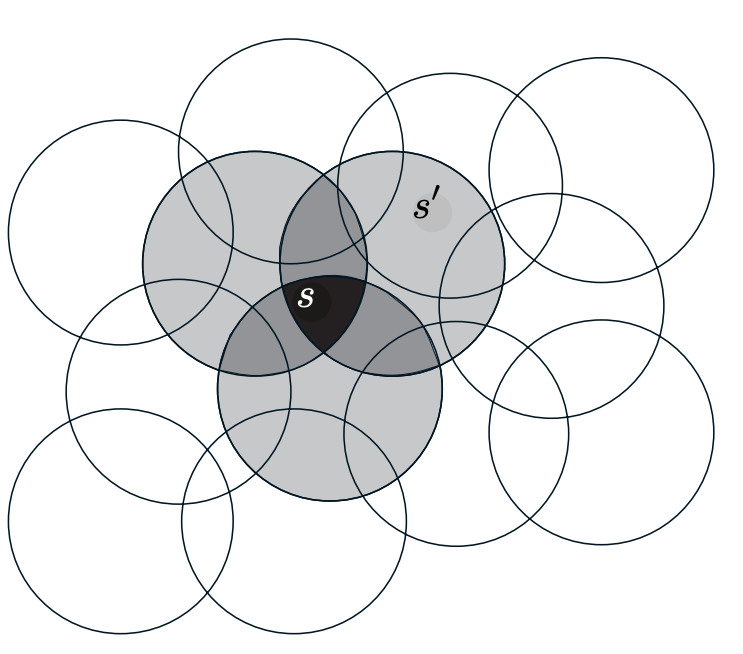
\includegraphics[width=0.75 \textwidth]{/chapter9_3}
	\caption{Coarse coding. Generalization from state $s$ to state $s_0$ depends on the number of their features whose receptive fields (in this case, circles) overlap. These states have one feature in common, so there will be slight generalization between them.}
	\label{fig: coarse coding}
\end{figure}

\subsubsection{Tile Coding}
Tile coding is similar to course coding, but now uses sets of overlapping, uniformly or asymmetrically distributed, tiles - Figure \ref{fig: tile coding}.  Tiles do not need to be squares, they can be irregular shapes, horizontal/vertical lines or log lines. Each affects the mode of generalisation in function approximation.

\begin{figure}[h!]
	\centering
	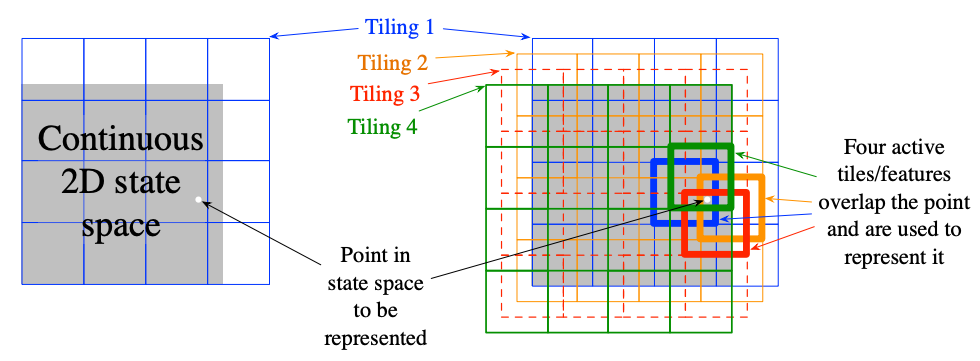
\includegraphics[width=\textwidth]{/chapter9_4}
	\caption{Multiple, overlapping grid-tilings on a limited two-dimensional space. These tilings are offset from one another by a uniform amount in each dimension.}
	\label{fig: tile coding}
\end{figure}

\subsubsection{Radial Basis Functions}
Radial Basis Functions (RBFs) are the natural extension of course coding to continuous-valued domains. Rather than a feature being either off or on (0 or 1), it can take any value in the interval [0,1]. Typical RBFs use Gaussian's to parametrise the distribution of the feature, which has centre state $c_i$ and width $\sigma_i$. The feature value therefore takes the form:
\begin{equation}
x_i(s) \doteq exp \left(-\frac{||s - c_i||^2}{2 \sigma_i^2}\right)
\end{equation}

Figure \ref{fig: rbf} shows the overlapping distribution of RBF features.

\begin{figure}[h!]
	\centering
	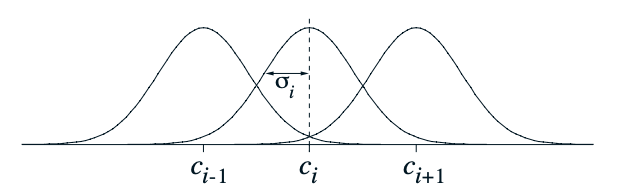
\includegraphics[width=\textwidth]{/chapter9_5}
	\caption{One-dimensional radial basis functions.}
	\label{fig: rbf}
\end{figure}

\subsection{Selecting Step-Size Parameters Manually}
Can we say in general how best to select $\alpha$ in our function approximator? A good rule of thumb for setting the step-size parameter of linear SGD methods is:
\begin{equation}
	\alpha \doteq (\tau \mathbb{E}[\textbf{x}^T\textbf{x}])^{-1}
\end{equation}

where \textbf{x} is a random feature vector chosen from the same distribution as input vectors will be in the SGD, and $\tau$ is the number of experiences within which you would like to learn.

\subsection{Nonlinear Function Approximation: Artificial Neural Networks}
Artificial Neural Networks (ANNs) have proven to be some of the best non-linear function approximators. We know plenty about them already, so here is some general points:
\begin{itemize}
\item ANNs overfit on training data, a problem mitigated by dropout.
\item Batch normalization involves normalising the output of hidden layers before passing them to the next layer, and performing this process on mini-batches of data. This improves the learning rates of the algorithms.
\end{itemize}

\subsection{Least-Squares TD}
Earlier, we established the TD fixed point as
\begin{align}
\textbf{w}_{TD} &\doteq \textbf{A}^-1\textbf{b}
\end{align}
where
\begin{equation}
\textbf{b} \doteq \mathbb{E}[R_{t+1} \textbf{x}_t] \in \mathbb{R}^d \; \; \text{and} \; \; \textbf{A} \doteq \mathbb{E}\left[\textbf{x}_t(\textbf{x}_t - \gamma \textbf{x}_{t+1})^T\right] \in \mathbb{R}^{d \times d}
\end{equation}
Instead of computing this solution iteratively, we could compute estimates of $A$ and $b$ and then directly compute the TD fixed point– this is the Least Squares TD algorithm (LSTD). It forms the estimates:
\begin{equation}
\hat{\textbf{A}_t} \doteq \sum_{k=0}^{t-1} \textbf{x}_k(\textbf{x}_k - \gamma \textbf{x}_{k+1})^T + \epsilon \textbf{I} \; \; \text{and} \; \; \hat{\textbf{b}_t} \doteq \sum_{k=0}^{t-1} R_{k+1}\textbf{x}_k
\end{equation}

where $\textbf{I}$ is the identity matrix, and $\epsilon \textbf{I}$, for some small $\epsilon > 0$ ensures that $\hat{\textbf{A}_t}$ is always invertible. It looks like both $\hat{\textbf{A}_t}$ and $\hat{\textbf{b}_t}$ should be divided by $t$ to achieve the expectation, but the $t$s cancel when used to calculate the the TD fixed point as 
\begin{equation}
\textbf{w}_{TD} \doteq \hat{\textbf{A}^-1}\hat{\textbf{b}}
\end{equation}

The inversion of the matrix usually requires $O(d^3)$ computation, but can be done with $O(d^2)$ using the \textit{Sherman-Morrison formula}. LSTD's lack of step size parameter means it never forgets, which is sometimes desirable, but often not in RL problems where both the environment and policy change with time.

\subsection{Memory-based Function Approximation}
So far we have been parametrising functions that approximate our value function, and these parameters are updated as we see more data. These are examples of \textit{parametric} models. An alternative approach is to store examples of transitions or rewards from one state to the next, and querying them when we arrive in a state, similar to the approach used in Dyna - Chapter 8. These are \textit{nonparametric} models or \textit{memory-based} function approximators, with examples including nearest neighbours, or locally weighted regressions, with the weights being proportional to the distance between current state and queried state.

Because these methods are \textit{local} approximations rather than \textit{global}, they allow us to somewhat overcome the curse of dimensionality, and only approximate the value function where it is required, rather than across the entire state space. For example, if we are working with a state space with $k$ dimensions, a tabular method , storing a global approximation requires memory exponential in $k$, whereas storing examples in a memory-based method requires only memory proportional to $k$, or linear in the number of examples $n$.

\subsection{Kernel-based Function Approximation}
In the previous subsection, we discussed weighted average regression, where the weight is proportional to some measure of distance. The function that assigns the weights in often called the \textit{kernel function} or simply a \textit{kernel} and takes the form $k: \mathcal{S} \times \mathcal{S} \rightarrow \mathbb{R}$ and is summarised by $k(s, s')$. Viewed  slightly differently, $k(s, s')$ is a measure of the strength of generalization from $s'$ to $s$.

\textit{Kernel regression} is the memory-based method that computes a kernel weighted average of the targets of \textit{all} examples stored in memory, assigning the result to the query state. If $\mathbb{D}$ is the set of stored examples, and $g(s')$ denotes the target for state $s'$ in a stored example, then the value function is
\begin{equation}
\hat{v}(s, \mathcal{D}) = \sum_{s' \in \mathcal{D}} k(s, s')g(s')
\end{equation}

The common kernel is the Gaussian radial basis function (RBF) as defined earlier and in the Gaussian Process literature. Kernel based methods allow us to operate in the high-dimensional feature space, only using stored examples, and without needing a complex, parametrised model. This is the so-called \textit{kernel trick} and is the basis of many modern machine learning methods.

\subsection{Looking Deeper at On-policy Learning: Interest and Emphasis}
Until now we have treated all encountered states equally, but it is likely that we will actually be more interested in some states that others. To deal with this, we introduce two new concepts called \textit{interest} and \textit{emphasis}. Interest is the degree to which we value an accurate estimate of the value of a given state, generally $I_t \in [0,1]$ and emphasis in a scalar that multiplies the learning update and thus emphasises or de-emphasises the learning done at time $t$. The emphasis is determined recursively from the interest by
\begin{equation}
M_t = I_t + \gamma^n M_{t-n}
\end{equation}

\subsection{Key Takeaways}
\begin{itemize}
\item \textit{Generalization} of RL systems is critical to be applicable to artificial intelligence and large engineering problems. Generalization is achieved by approximating the value function using various techniques.
\item We defined the the prediction objective $\bar{VE}(\textbf{w})$, called the \textit{mean squared value error}, which provides a rational basis for comparing different function approximators.
\item Most techniques use stochastic gradient descent (SGD) to find the set of weight parameters than minimise $\bar{VE}(\textbf{w})$
\item Linear methods can be proven to converge to the globally optimum weight vector under certain conditions. 
\item Features, used to build linear methods, can take many forms, including: polynomials, fouriers, coarse codings, tile codings, and RBFs.
\item Artificial NNs have been proven to be potentially the most effective nonlinear function approximator.
\item Instead of using \textit{parametric} function approximators, \textit{nonparamteric} models can be used that predict values based on the distance of a current state to past observed next states for which we have some stored values, or state representations.
\item \textit{Interest}and \textit{Emphasis} allow us to focus the function approximation on parts of the state space where we would value more accurate estimates.
\end{itemize}





\section{On-policy Control with Approximation}
\section{*Off-policy Methods with Approximation}
Notes on this section tbc.
\section{Eligibility Traces}
\begin{itemize}
	\item Eligibility traces are an alternative way of performing $n$-step TD prediction or control.
	\item $n$-step methods can be seen as \textit{forward view} algorithms that look at future rewards seen from some state and update the state value accordingly. Eligibility traces are \textit{backward view} methods that update previous state values based on how \textit{responsible} we think they were for the reward we have just obtained.
	\item They are more computationally efficient than $n$-step methods because they don't have to store the last $n$ feature vectors, but instead store one  \textit{trace} vector.
\end{itemize}

\subsection{The $\lambda$-return}
In Chapter 7 we derived the $n$-step return $G_{t:t+n}$ and used it to make updates to the state value. What if instead of using one $n$-step return, we took a weighted average of every $n$-step return? This is the $\lambda$-return and is called a \textit{compound update}, rather than a \textit{component update} in the $n$-step case. We could, for example, take the mean of the 2-step and 4-step updates, the backup diagram for which is shown in Figure \ref{fig: 12_1}.
\begin{figure}[h!]
	\centering
	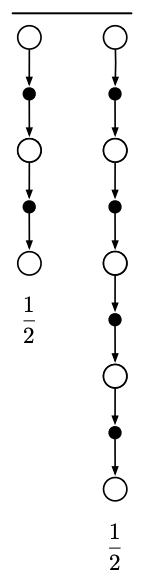
\includegraphics[width=0.1\textwidth]{/chapter12_1}
	\caption{Backup diagram for compound update for 2-step and 4-step returns}
	\label{fig: 12_1}
\end{figure}

The TD($\lambda$) algorithm generalises this approach such that each $n$-step update is weighted proportionally to $\lambda^{n-1}$ (where $\lambda \in [0, 1]$). The $\lambda$-\textit{return} in the state-based form is given by
\begin{equation} \label{eq: lambda return}
G_t^\lambda \doteq (1-\lambda) \sum_{n=1}^{\infty} \lambda^{n-1}G_{t:t+n}
\end{equation}
and the backup diagram for the algorithm is given in Figure \ref{fig: 12_2}, the decaying weighting factor is given in Figure \ref{fig: 12_3}.

\begin{figure}
	\centering
	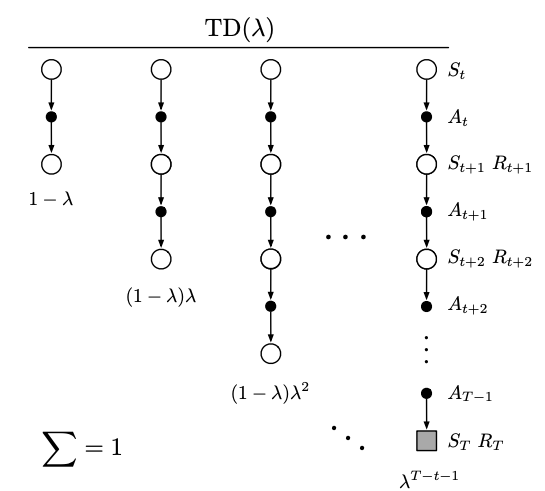
\includegraphics[width=0.6\textwidth]{/chapter12_2}
	\caption{The backup digram for TD($\lambda$). If $\lambda$ = 0, then the overall update reduces to its first component, the one-step TD update, whereas if $\lambda$ = 1, then the overall update reduces to its last component, the Monte Carlo update.}
	\label{fig: 12_2}
\end{figure}

\begin{figure}
	\centering
	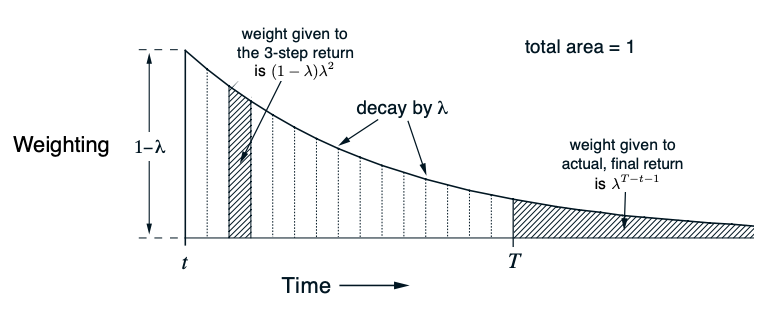
\includegraphics[width=\textwidth]{/chapter12_3}
	\caption{Weighting given in the $\lambda$-return to each of the n-step returns.}
	\label{fig: 12_3}
\end{figure}

Intuitively this algorithm makes sense. We give more responsibility for our rewards to recently selected actions and less to older selected actions, but nonetheless take into account all previously taken actions. Crucially, this algorithm is forward view, the episode is completed then we return to the first step and update based on the weighted average of all $n$-step returns received thereafter, cycling through each state.

\subsection{TD($\lambda$)}
In TD($\lambda$) the eligibility trace is first initialized to 0, and then incremented at each step by the value gradient and fades according to $\lambda$
\begin{align} \label{z}
\textbf{z}_{-1} &\doteq \textbf{0} \\
\textbf{z}_t &\doteq \gamma \lambda \textbf{z}_{t-1} + \nabla \hat{v}(S_t, \textbf{w}_t)
\end{align}

here the value gradient is effectively a proxy for the state visited i.e. bump up the eligibility at these weights because a state corresponding to these weights has been visited recently. We know the TD error for state-value prediction is
\begin{equation}
\delta_t \doteq R_{t+1} + \gamma \hat{v}(S_{t+1}, \textbf{w}_t) - \hat{v}(S_t, \textbf{w}_t)
\end{equation}

and the weight vector in TD($\lambda$) is updated in proportion to the TD error and the eligibility trace
\begin{equation}
\textbf{w}_{t+1} \doteq \textbf{w}_t + \alpha \delta_t \textbf{z}_t
\end{equation}

The algorithm for semi-gradient TD($\lambda$) is given in Figure \ref{fig: 12_4}
\begin{figure}
	\centering
	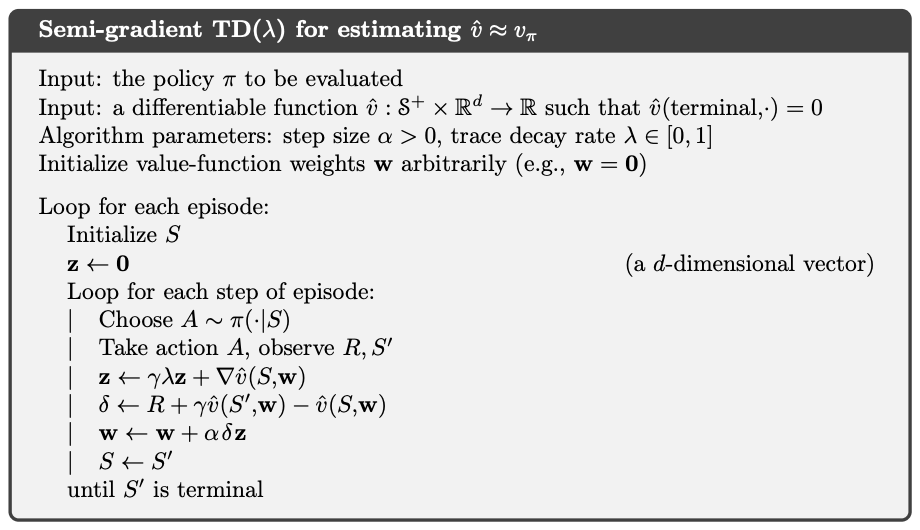
\includegraphics[width=0.8\textwidth]{/chapter12_4}
	\caption{Pseudocode for semi-gradient TD($\lambda$)}
	\label{fig: 12_4}
\end{figure}

To understand TD($\lambda$) better lets consider the extreme cases of $\lambda = 0$ and $\lambda = 1$. In the former, the algorithm becomes one step returns as per TD(0) discussed in chapter 6. In the later we get Monte Carlo returns where every single previous state is updated with the return, but discounted by $\gamma$. (Note: this gives insight as to why $\gamma$ is still retained in equation \ref{z}). The advantage of this kind of Monte Carlo return, as compared with the normal MC return discussed in chapter 5, is that it can be performed \textit{online} rather than waiting for the end of the episode before backpropogating the returns.

\subsection{$n$-step Truncated $\lambda$-return Methods}
The off-line $\lambda$-return algorithm, which uses the $\lambda$-return (Equation \ref{eq: lambda return}), is an important ideal but of little use in the episodic case (because we have to wait until the end of the episode before we make any updates), nor the continuing case (because it cannot be calculated for arbitrarily large $n$). Instead we can use the truncated $\lambda$-return which halts the return calculation at some horizon $h$:
\begin{equation} \label{eq: horizon}
G_{t:h}^\lambda \doteq (1 - \lambda) \sum_{n=1}^{h - t - 1} \lambda^{n-1} G_{t:t+n} + \lambda^{h-t-1}G_{t:h}, \; \; \; 0 \leq t < h \leq T
\end{equation}

\subsection{Redoing Updates: Online $\lambda$-return Algorithm}
The problem with the algorithm described in the last section is the choice of truncation parameter $n$. If it is too small, then we do not get the benefit of the offline $\lambda$-return algorithm that uses all $n$ step updates from an episode, and if it is too large then we cannot learn quickly online. We can, in principle, get the best of both using the \textit{online $\lambda$-return algorithm}, but we pay for this with computational complexity.

For every step we take in an episode, we recalculate the $\lambda$-return for the whole episode, where our current step acts as horizon $h$ in equation \ref{eq: horizon}. We are then making increasingly accurate updates to states as we move through the episode, but the number of calculations required at each step scales with $n$. The updates are given in Figure \ref{fig: 12_5}.
\begin{figure}
	\centering
	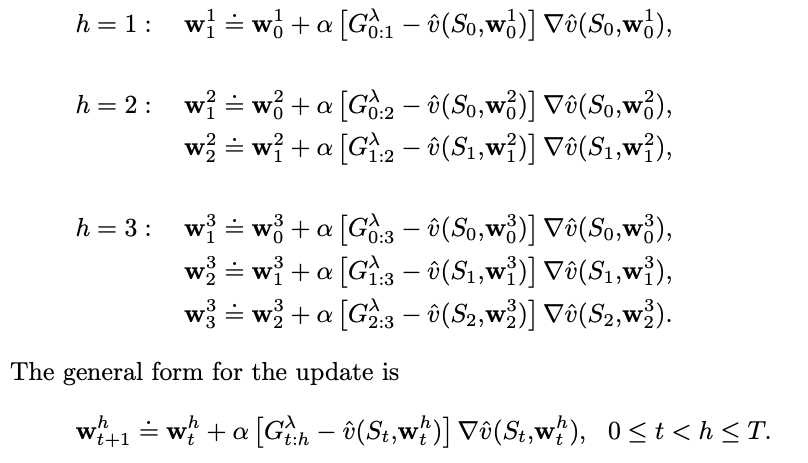
\includegraphics[width=0.6\textwidth]{/chapter12_5}
	\caption{Online $\lambda$-return updates for the first three steps of an episode}
	\label{fig: 12_5}
\end{figure}

In general, online $\lambda$-return performs better than off $\lambda$-return because it has had more, informative updates the weight vector used for bootstrapping throughout the episode. Note: this is a forward view algorithm, we keep updating state values by looking at a stream of future rewards as they are updated 

\subsection{True Online TD($\lambda$)}
\begin{itemize}
\item We can produce a backward view version of the online $\lambda$-return algorithm presented in the last section that uses eligibility traces, called True Online TD($\lambda$).
\item Because of a trick with the weight matrix, where we only need to keep the last weight vector from all the updates at the last time step, the computational complexity of True Online TD($\lambda$) matches TD($\lambda$).
\item The pseudocode for True Online TD($\lambda$) is given in Figure \ref{fig: 12_6}.
\end{itemize}
\begin{figure}
	\centering
	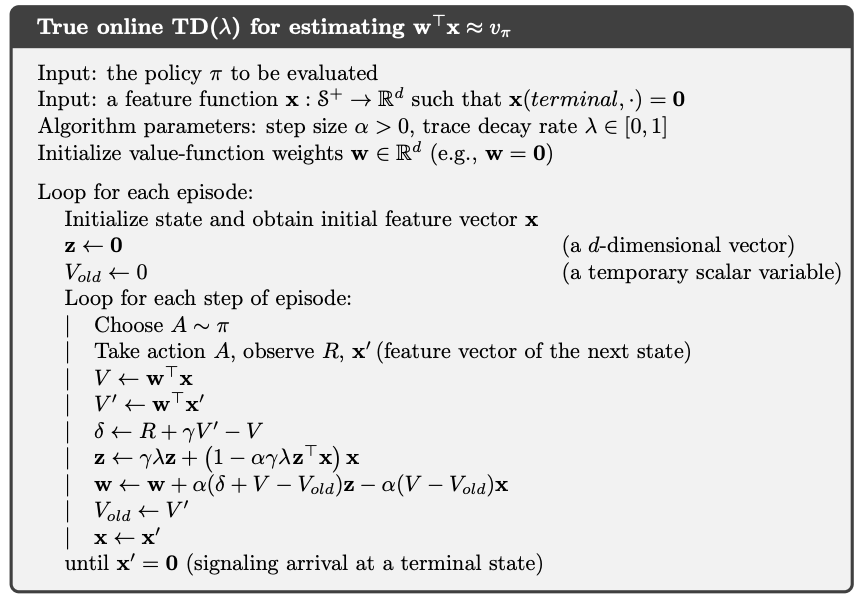
\includegraphics[width=0.8\textwidth]{/chapter12_6}
	\caption{True Online TD($\lambda$)for estimating $\textbf{w}^T\textbf{x} \approx v_\pi$}
	\label{fig: 12_6}
\end{figure}

\subsection{SARSA($\lambda$)}
We can extend the ideas discussed in this chapter (i.e. eligibility traces) to the action-value, forward-view case readily, producing the SARSA($\lambda$) algorithm. The full list of equations required for SARSA($\lambda$) are detailed below. First we need the action-value form of the $n$-step return
\begin{equation}
G_{t:t+n} \doteq R_{t+1} + \cdots + \gamma^{n-1} R_{t+n} + \gamma^n \hat{q}(S_{t+n}, A_{t+n}, \textbf{w}_{t+n-1}), \; \; \; t+n < T,
\end{equation}
with $G_{t:t+n} \doteq G_t$ if $t+n \geq T$. The action-value form of the offline $\lambda$-return algorithm simply use $\hat{q}$ rather than $\hat{v}$:

\begin{equation}
\textbf{w}_{t+n} \doteq \textbf{w}_{t+n-1} + \alpha \left[G_{t}^\lambda - \hat{q} (S_t, A_t, \textbf{w}_{t+n-1})\right] \nabla \hat{q}(S_t, A_t, \textbf{w}_{t+n-1}), \; \; \; t=0, \ldots, T-1
\end{equation}
where $G_{t}^\lambda \doteq G_{t: \infty}^\lambda$.  The algorithm has the same update rule as given earlier for TD($\lambda$)
\begin{equation}
\textbf{w}_{t+1} \doteq \textbf{w}_t + \alpha \delta_t \textbf{z}_t
\end{equation}
except it uses the action-value form of the TD error:
\begin{equation}
\delta_t \doteq R_{t+1} + \gamma \hat{q}(S_{t+1}, A_{t+1}, \textbf{w}_t) - \hat{q}(S_t, A_{t}, \textbf{w}_t),
\end{equation}
and the action-value form of the eligibility trace:
\begin{align} \label{z}
\textbf{z}_{-1} &\doteq \textbf{0} \\
\textbf{z}_t &\doteq \gamma \lambda \textbf{z}_{t-1} + \nabla \hat{q}(S_t, A_{t}, \textbf{w}_t), \; \; \; 0 \leq t \leq T.
\end{align}

Complete pseudocode for the algorithm is given in Figure \ref{fig: 12_7}.

\begin{figure}
	\centering
	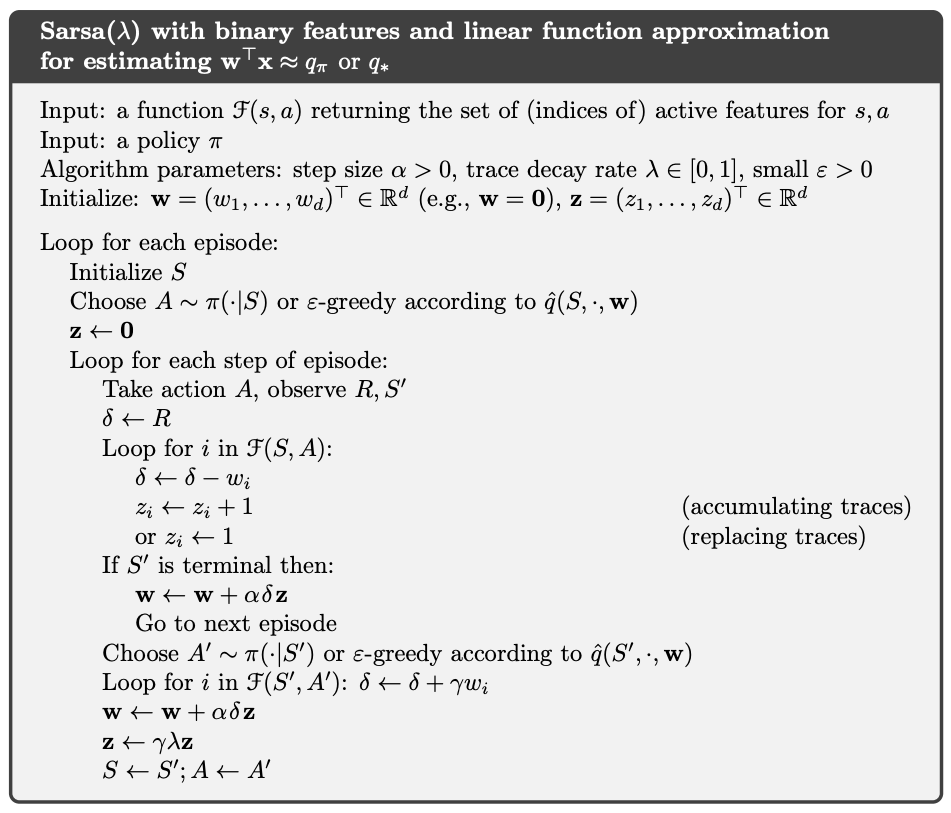
\includegraphics[width=0.8\textwidth]{/chapter12_7}
	\caption{SARSA($\lambda$) with binary features and linear function approximation for estimating $w^T \approx q_\pi or q_*$}
	\label{fig: 12_7}
\end{figure}

A compelling visual description of the different SARSA algorithms reviewed thus far is given in Figure \ref{fig: 12_8}. The SARSA($\lambda$) updates make the most intuitive sense. It is the actions closest to the final reward where we can be most confident in their value, actions prior to the goal may have had a direct effect in producing the reward, but the distance between action and target means there is uncertainty in how much that action affected the final outcome. Consequently, updating the values of these actions more conservatively appears rational. SARSA($\lambda$) proves the most efficient and learning optimal policies in these settings for this reason.

To explain clearly the intuition behind this algorithm we refer back to Figure \ref{fig: 12_3}. If we imagine ourselves in the first state and observe the weight we give to all forthcoming updates, we see that we give the bulk of the weight to the initial rewards we receive (0 in the gridworld) and the least weight to the final return at time $T$. Equally, if we are in the final state prior to termination, we give most weight to the next-step rewards (1 in the gridworld). This creates the fading reward traces shown in Figure \ref{fig: 12_7}.

\begin{figure}
	\centering
	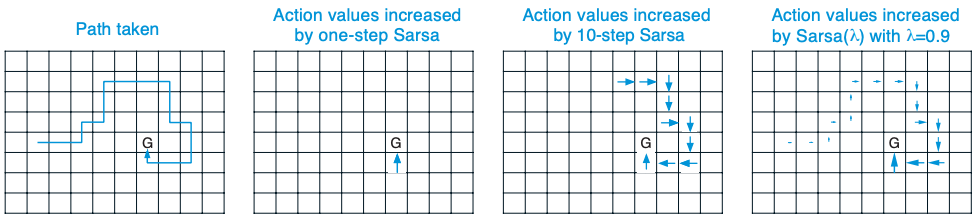
\includegraphics[width=0.8\textwidth]{/chapter12_8}
	\caption{4 SARSA algorithms tackling the gridworld task}
	\label{fig: 12_8}
\end{figure}

\subsection{Variable $\lambda$ and $\gamma$}
We can amend $\lambda$, the eligibility trace parameter, and $\gamma$, the discounting parameter, to vary with state rather than be constants throughout an episode. That is, $\lambda$ and $\gamma$ are now state-dependent and denoted $\lambda_t$ and $\gamma_t$. This creates a further layer of generalisation not yet seen. The return is now defined more generally as
\begin{align}
	G_t &\doteq R_{t+1} + \gamma_{t+1}G_{t+1} \\
	&= R_{t+1} + \gamma_{t+1}R_{t+2} + \gamma_{t+1}\gamma_{t+2}R_{t+3} + \cdots \\
	&= \sum_{k=t}^{\infty} \left(\prod_{i=t+1}^{k} \gamma_i\right) R_{k+1} \\
\end{align}

\subsection{Off-policy Traces with Control Variates}
To generalise to the off-policy case we need to bring back ideas from importance sampling. This section, and associated derivations, are long, but eventually we arrive at a new eligibility trace
\begin{equation}
\textbf{z}_t \doteq \gamma_t \lambda_t \rho_t \textbf{z}_{t-1} + \nabla \hat{q}(S_t, A_t, \textbf{w}_t), 
\end{equation}
where $\rho_t = \frac{\pi(A_t | S_t)}{b(A_t | S_t)}$ is the single-step importance sampling ratio.

\subsection{Watkins's Q($\lambda$) to Tree-Backup($\lambda$)}
Q-learning and Tree-backups can be extended to the eligibility trace setting too, and are called Watkins's Q($\lambda$) and Tree-backup($\lambda$) respectively. Their backup diagrams are shown in Figures \ref{fig: 12_9} and \ref{fig: 12_10}. In Q($\lambda$) we continue to include weighted $n$-step rewards whilst greedy actions are selected, but when a non-greedy action is selected on-policy the cumulative reward terminates with an expectation at that state.

\begin{figure}
	\centering
	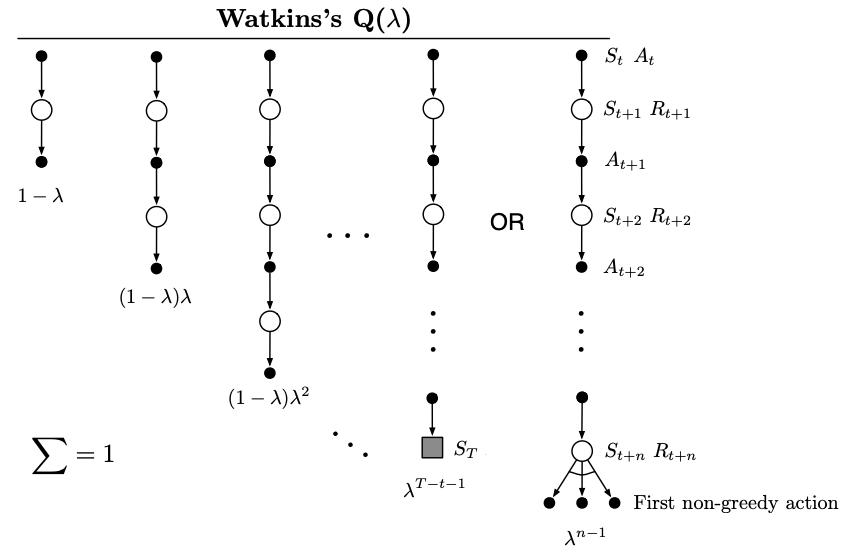
\includegraphics[width=0.8\textwidth]{/chapter12_9}
	\caption{The backup diagram for Watkins’s Q($\lambda$). The series of component updates ends either with the end of the episode or with the first non-greedy action, whichever comes first.}
	\label{fig: 12_9}
\end{figure}

\begin{figure}
	\centering
	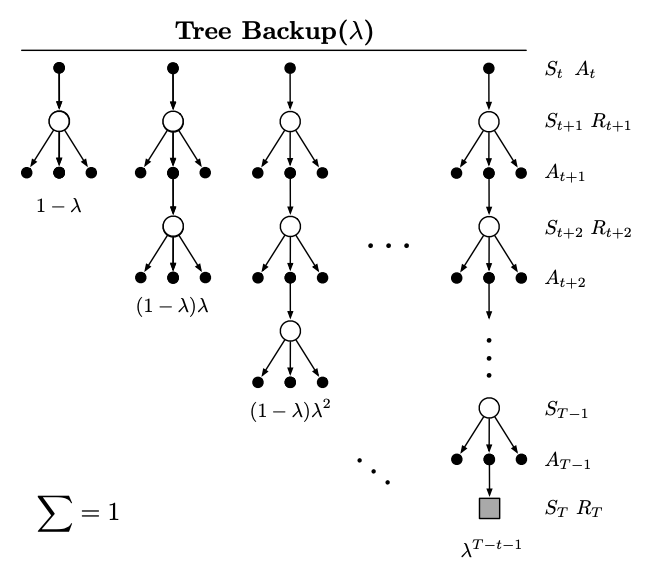
\includegraphics[width=0.7\textwidth]{/chapter12_10}
	\caption{The backup diagram for the $\lambda$ version of the Tree Backup algorithm.}
	\label{fig: 12_10}
\end{figure}

\subsection{Implementation Issues}
In the tabular setting, it would appear that every state-value instance would need to be updated at every timestep. This is a problem for implementation on traditional serial computers. Fortunately, for typical values of $\lambda$ and $\gamma$, almost all state have eligibility traces near zero. In practice, therefore, we only need to update the states for which the update is some margin bigger than zero, decreasing the complexity of the system. Function approximation, like ANNs, reduce the complexity of eligibility-based algorithms too.

\subsection{Key Takeaways}
\begin{itemize}
\item Eligibility traces allow us to walk the continuum between one-step methods and Monte Carlo in a similar way to the $n$-step methods discussed in chapter 7. They are, however, more general, and learn value functions more quickly.
\item Monte Carlo methods are good in non-Markov environments, because their rewards are unbiased by bootstrapping. Eligibility traces have the same property. They are most useful for environments that have long-delayed rewards and are non-Markov.
\item Eligibility traces use significantly more computation than $n$-step methods, but in return they offer significantly faster learning, particularly when rewards are delayed by many steps. Thus they can be particularly effective in \textbf{low data settings}, and not effective when data can be acquired cheaply via a simulator. When data is cheap, the challenge is processing that data as quickly as possible, and typically, that means using one-step methods like Q-learning.
\item $\lambda$-return is forward view and TD($\lambda$) is backward view.
\end{itemize}



\section{Policy Gradient Methods}
Instead of learning action-value estimates, and deriving a policy thereafter, we will now parameterize a policy directly depending on its performance. Our policy is now $\pi(a|s, \boldsymbol{\theta})$ representing the probability of taking action $a$ in state $s$ given parameter vector $\theta \in \mathbb{R}^{d'}$. \textit{Actor-critic} methods learn both a parameterised policy (the actor) and a parameterised value function estimate (the critic)

The policy parameter update is therefore
\begin{equation}
\boldsymbol{\theta}_{t+1} = \boldsymbol{\theta}_{t} + \alpha \nabla \hat{J(\boldsymbol{\theta}_{t})} 
\end{equation}

where $\hat{J(\boldsymbol{\theta}_{t})}$ is a stochastic estimate whose expectation approximates the gradient of the performance measure with respect to its argument $\boldsymbol{\theta}_{t}$.

\subsection{Policy Approximation and its Advantages}
\begin{itemize}

\item The policy can be parameterised in any way as long as $\pi(a|s, \boldsymbol{\theta})$ is differentiable.
\item If the action-space is discrete and not too large, then a natural and common kind of parameterisation is to form numerical preferences $h(s,a, \boldsymbol{\theta}) \in \mathbb{R}$ for each state-action pair. The actions with the highest preferences in each state are given the highest probabilities of being selected, for example, according to an exponential soft-max distribution:
\begin{equation}
\pi(a|s, \boldsymbol{\theta}) \doteq \frac{e^{h(s,a,\boldsymbol{\theta})}}{\sum_{b}e^{h(s,b,\boldsymbol{\theta})}}
\end{equation}.

\item We call this kind of policy parameterisation \textit{soft-max in action preferences}. An advantage of parameterising policies according to soft-max action preferences is that the approximate policy can approach a determinisitc policy, whereas with $\epsilon$-greedy action selection over action values there is always an $\epsilon$ probability of selecting a random action.
\item A second advantage of soft-max action preferences is that we can now select actions with arbritrary probabilities, rather than the greedy action selected most of the time and all other actions given probability of selection $\epsilon / |\mathcal{A}|$. This is useful in environments with imperfect information, where it is useful to act stochastically e.g. when bluffing in poker it is useful to do so randomly to unnerve an opponent.
\item Often the most important reason for using a policy-gradient method is that we can inject prior knowledge about the system in the RL agent.
\end{itemize}

\subsection{The Policy Gradient Theorem}
We define performance in the episodic case as
\begin{equation}
J(\boldsymbol{\theta}) \doteq v_{\pi\theta(s_0)},
\end{equation}
where $v_{\pi\theta(s_0)}$ is the true value function for $\pi_{\boldsymbol{\theta}}$, the policy determined by $\boldsymbol{\theta}$. And $s_0$ is some non-random start state. The policy gradient theorem then establishes that
\begin{equation} \label{eq: policy gradient theorem}
\nabla J(\boldsymbol{\theta}) \propto \sum_{s} \mu(s) \sum_{a} q_\pi(s,a) \nabla \pi(a|s, \boldsymbol{\theta})
\end{equation}

where $\mu$ is the on-policy distribution under $\pi$ as discussed previously i.e. the theorem is a sum over states weighted by how often the states occur under the target policy $\pi$. We can use this to approximate gradient ascent without access to the derivative of the state distribution.

\subsection{REINFORCE: Monte Carlo Policy Gradient}
REINFORCE is a method for updating our policy parameters based on episodic returns from states $G_t$. We update the parameters in the direction of actions that yielded highest rewards. Recall from Equation \ref{eq: policy gradient theorem} that the policy gradient theorem is a weighted sum of over states which is the same as an expectation over states:
\begin{align}
\nabla J(\boldsymbol{\theta}) &\propto \sum_{s} \mu(s) \sum_{a} q_\pi(s,a) \nabla \pi(a|s, \boldsymbol{\theta}) \\
&= \mathbb{E}_\pi \left[\sum_{a} q_\pi(S_t, a) \nabla \pi(a, S_t, \boldsymbol{\theta})  \right]
\end{align}

We can arrive at REINFORCE by replacing the sum over the random variable's possible values by an expectation under $\pi$, and then sampling the expectation. We multiply and divide the summed terms by $\pi(a | S_t, \boldsymbol{\theta})$:
\begin{align}
\nabla J(\boldsymbol{\theta}) &\propto \mathbb{E}_\pi \left[\sum_{a} \pi(a | S_t, \boldsymbol{\theta}) q_\pi(S_t, a) \frac{\nabla \pi(a, S_t, \boldsymbol{\theta})}{\pi(a, S_t, \boldsymbol{\theta})} \right] \\
&= \mathbb{E}_\pi \left[q_\pi(S_t, A_t) \frac{\nabla \pi(A_t, S_t, \boldsymbol{\theta})}{\pi(A_t, S_t, \boldsymbol{\theta})} \right] \; \; \; \text{(replacing $a$ by the sample $A_t \sim \pi$)} \\
&= \mathbb{E}_\pi \left[G_t \frac{\nabla \pi(A_t, S_t, \boldsymbol{\theta})}{\pi(A_t, S_t, \boldsymbol{\theta})} \right] \; \; \; \text{(because $\mathbb{E}_\pi \left[G_t|S_t, A_t\right] = q_\pi(S_t, A_t)$)} \\
\end{align}

The last expression is what we need: a quantity that can be sampled on each time step whose expectation is proportional to the gradient. We now arrive at the REINFORCE update
\begin{equation}
\boldsymbol{\theta}_{t+1} \doteq \boldsymbol{\theta}_{t} + \alpha G_t \frac{\nabla \pi(A_t, S_t, \boldsymbol{\theta})}{\pi(A_t, S_t, \boldsymbol{\theta})}
\end{equation}

This update makes intuitive sense. The gradient term represents the direction in parameter space that most increases the probability of taking that same action again in the future. In effect, the gradient distil the policy approximation down to the weights that were most responsible for the action taken, from there we can affect these weights based on how much we valued the action. If the action yielded high reward $G_t$, then we boost the weights in proportion to the reward, and if this action has low probability of being taken under the current policy (the denominator $\pi(A_t, S_t, \boldsymbol{\theta})$) then the weights are further boosted. Alternatively, if the action is taken often, and yields low reward, we make little adjustment to the weights, lowering their impact on the policy approximation in the long run as other weights receive boosts.

Note this is a monte carlo algorithm, using complete returns as updates, meaning it is only well defined in the episodic case, and can have high variance causing slow learning. The pseudocode for REINFORCE is given in Figure \ref{fig: 13_1}.
\begin{figure}
	\centering
	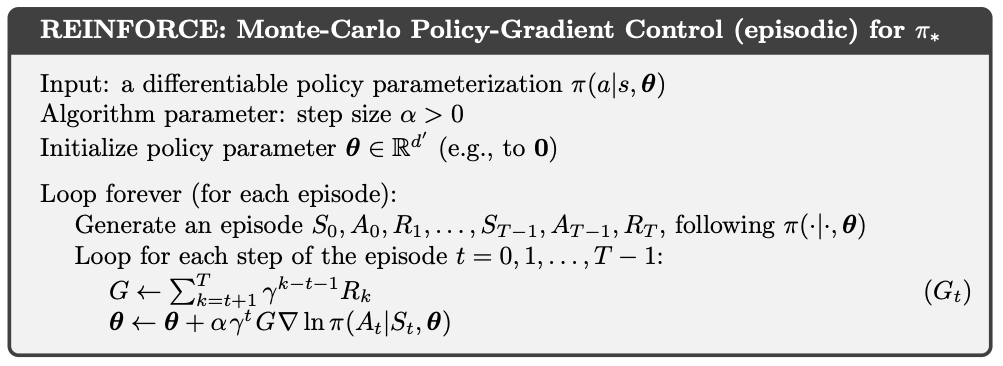
\includegraphics[width=\textwidth]{/chapter13_1}
	\caption{Pseudocode for REINFORCE: monte carlo policy-gradient control (episodic) for $\pi_*$}
	\label{fig: 13_1}
\end{figure}

\subsection{REINFORCE with Baseline}
The policy gradient theorem can be generalized to include a comparison of the action value to an arbitrary \textit{baseline} $b(s)$:
\begin{equation}
\nabla J(\boldsymbol{\theta}) \propto \sum_{s} \mu(s) \sum_{a} \left( q_\pi(s,a) - b(s) \right) \nabla \pi(a|s, \boldsymbol{\theta})
\end{equation}

We do this because it can help us reduce the variance of our results, which speeds learning. By comparing our observed result with some state-dependent baseline, we get a feel for how different the observed value is from what we expected. Thus, we arrive at a lower variance REINFORCE update as
\begin{equation}
\boldsymbol{\theta}_{t+1} \doteq \boldsymbol{\theta}_{t} + \alpha \left(G_t - b(S_t) \right) \frac{\nabla \pi(A_t, S_t, \boldsymbol{\theta})}{\pi(A_t, S_t, \boldsymbol{\theta})}
\end{equation}

The natural baseline is an estimate of the state value, $\hat{v}(S_t, \textbf{w})$, which we can learn as discussed in previous chapters. This method significantly speeds up learning as shown in Figure \ref{fig: 13_2}.
\begin{figure}
	\centering
	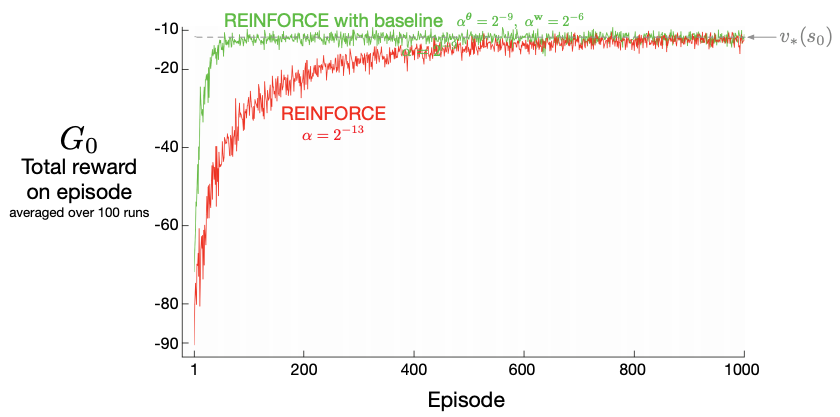
\includegraphics[width=\textwidth]{/chapter13_2}
	\caption{Adding a baseline to REINFORCE can make it learn much faster, as illustrated here on the short-corridor gridworld (Example 13.1). The step size used here for plain REINFORCE is that at which it performs best.}
	\label{fig: 13_2}
\end{figure}

\subsection{Actor-Critic Methods}
\begin{itemize}
\item The REINFORCE method uses the state-value function as a baseline for comparing true return from a state with what we expected the return to be. Because this comparison is made prior to action selection, we cannot use it to directly evaluate actions. In actor-critic methods, the state-value function is applied also to the \textit{second} state of the transition, which, when discounted and added to the one-step reward, constitutes the one-step return $G_{t:t+1}$.
\item When the state-value function is used in this way it is called the \textit{critic} and the policy is the \textit{actor}.
\item One-step actor-critic methods replace the full return of REINFORCE with the one-step return (and use a learned state-value function as the baseline) as follows:
\begin{align}
\boldsymbol{\theta}_{t+1} &\doteq \boldsymbol{\theta}_{t} + \alpha \left(G_{t:t+1} - \hat{v}(S_t, \textbf{w}) \right) \frac{\nabla \pi(A_t, S_t, \boldsymbol{\theta})}{\pi(A_t, S_t, \boldsymbol{\theta})} \\
&=  \boldsymbol{\theta}_{t} + \alpha \left(R_{t+1} + \gamma \hat{v}(S_{t+1}, \textbf{w}) - \hat{v}(S_t, \textbf{w})  \right) \frac{\nabla \pi(A_t, S_t, \boldsymbol{\theta})}{\pi(A_t, S_t, \boldsymbol{\theta})} \\
&=  \boldsymbol{\theta}_{t} + \alpha \delta_t \frac{\nabla \pi(A_t, S_t, \boldsymbol{\theta})}{\pi(A_t, S_t, \boldsymbol{\theta})} 
\end{align}
\item The pseudocode for one-step actor-critic is given in Figure \ref{fig: 13_3}, and it can be extended to include eligibility traces from Chapter 11 as shown in Figure \ref{fig: 13_4}.
\end{itemize}

\begin{figure}
	\centering
	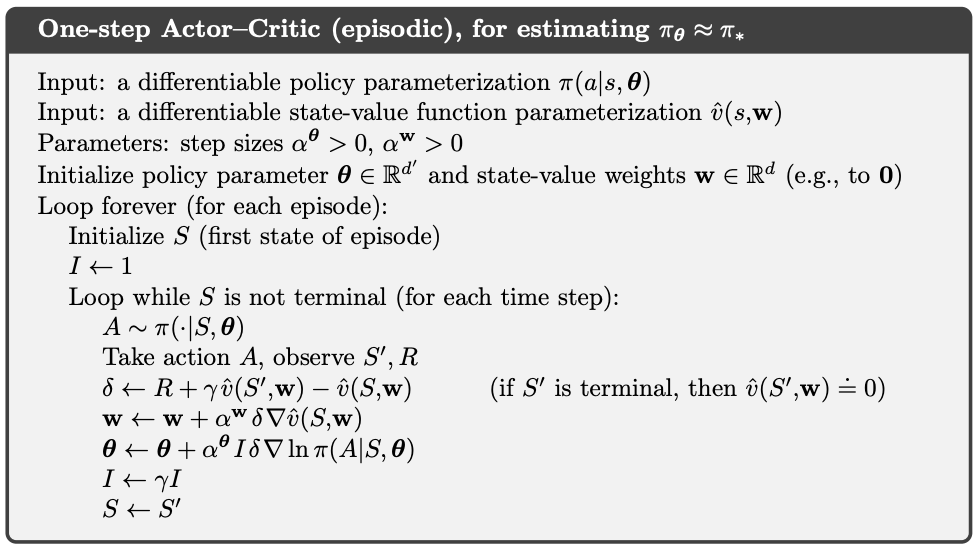
\includegraphics[width=0.8\textwidth]{/chapter13_3}
	\caption{Pseudocode for one-step actor-critic}
	\label{fig: 13_3}
\end{figure}

\begin{figure}
	\centering
	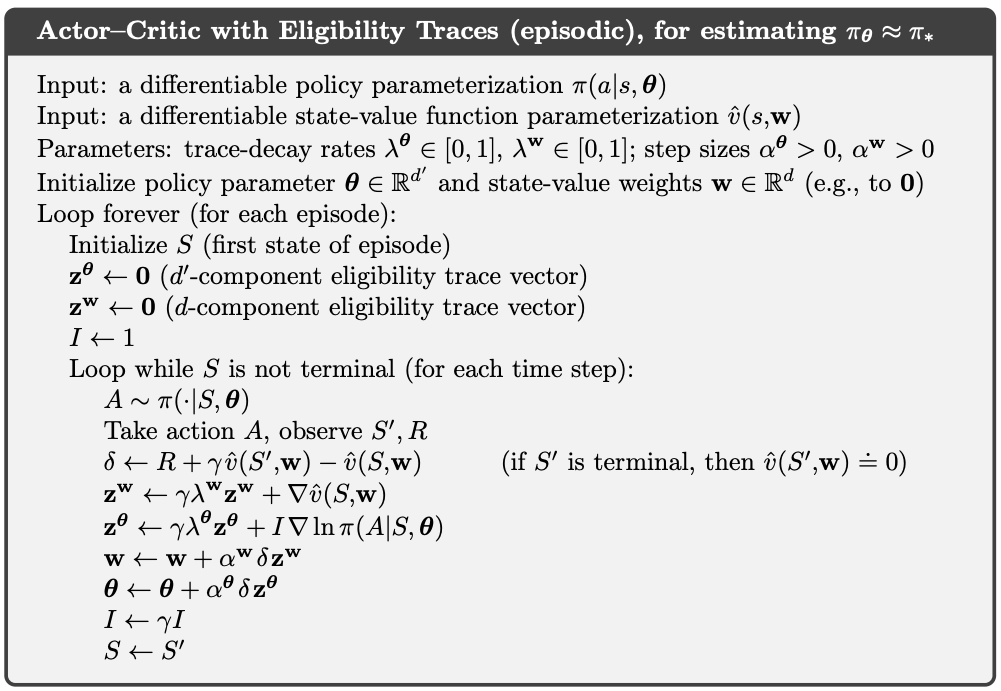
\includegraphics[width=0.8\textwidth]{/chapter13_4}
	\caption{Pseudocode for one-step actor-critic with eligibility traces}
	\label{fig: 13_4}
\end{figure}

\subsection{Policy Gradient for Continuing Problems}
As discussed in Chapter 10, for continuing problems without episode boundaries we need to define the performance in terms of average rate of reward per time step:
\begin{align}
J(\boldsymbol{\theta}) &\doteq r(\pi) \\
&= \lim_{t \rightarrow \infty} \mathbb{E} [R_t | S_0, A_{0:t-1} \sim \pi] \\
&= \sum_{s} \mu(s) \sum_{a} \pi(a | s) \sum_{s', r} p(s', r | s, a) r \\ 
\end{align}

We need to remember that in the continuing case, we define values $v_\pi(s) \doteq \mathbb{E}[G_t, S_t = s]$ and $q_\pi(s,a) \doteq \mathbb{E}[G_t, S_t = s, A_t = a]$ w.r.t the differential return:
\begin{equation}
G_t \doteq R_{t+1} - r(\pi) + R_{t+2} - r(\pi) + R_{t+3} - r(\pi) + \cdots
\end{equation}
Pseudocode for the continuing case is given in Figure \ref{fig: 13_5}.

\begin{figure}
	\centering
	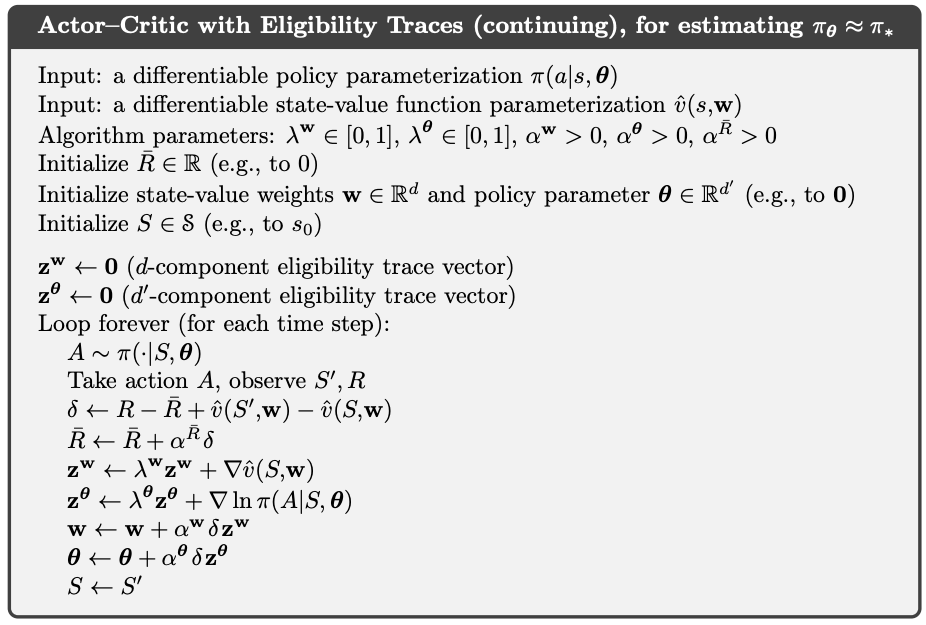
\includegraphics[width=0.8\textwidth]{/chapter13_5}
	\caption{Pseudocode for one-step actor-critic with eligibility traces, continuing case}
	\label{fig: 13_5}
\end{figure}

\subsection{Policy Parameterisation for Continuous Actions}
For state-spaces with huge numbers of actions, or continuous action spaces with infinite numbers of actions, we do not need to learn the probability of selecting each of these many actions, we can instead learn the parameters of the distribution over actions given a state. The probability density function for the normal distribution is conventionally written
\begin{equation}
p(x) \doteq \frac{1}{\sigma \sqrt{2 \pi}}exp\left(-\frac{(x - \mu)^2}{2 \sigma^2}\right)
\end{equation}

where $\mu$ and $\sigma$ are the mean and standard deviation of the normal distribution. Note $p(x)$ is the density of the probability, \textit{not} the probability itself. As such it can be greater than 1; it is the area under the graph that must sum to 1. One can take the integral between two values of $x$ to arrive at the probability of $x$ falling within that range. The policy parameterisation therefore becomes:
\begin{equation}
\pi(a | s, \boldsymbol{\theta}) \doteq \frac{1}{\sigma(s, \boldsymbol{\theta}) \sqrt{2 \pi}}exp\left(-\frac{(x - \mu(s, \boldsymbol{\theta}))^2}{2 \sigma(s, \boldsymbol{\theta})^2}\right)
\end{equation}

where $\mu : \mathcal{S} \times \mathbb{R}^{d'} \rightarrow \mathbb{R}$ and $\sigma : \mathcal{S} \times \mathbb{R}^{d'} \rightarrow \mathbb{R^+}$ i.e. they are both matrices of with dimensions equal to the number of states times the number of dimensions of the feature vector defining the policy. To from the policy approximator we need to split the policy's parameter vector into two parts, $\boldsymbol{\theta} = [\boldsymbol{\theta}_\mu, \boldsymbol{\theta}_\sigma]^T$. The mean can be approximated as a linear function, but the standard deviation must always be positive and is better approximated as the exponential of a linear function. Thus
\begin{equation}
\mu(s, \boldsymbol{\theta}) \doteq \boldsymbol{\theta}_\mu^T \textbf{x}_\mu(s) \; \; \; \text{and} \; \; \; \sigma(s, \boldsymbol{\theta}) \doteq exp\left(\boldsymbol{\theta}_\sigma^T \textbf{x}_\sigma(s)\right)
\end{equation}

\subsection{Key Takeaways}
\begin{itemize}
\item Prior to this chapter, actions had been selected by consulting an action-value function that informed us of how valuable actions were in given states at reaching our goal. Here, we instead parameterised policies directly, updating our approximations by reviewing the rewards received after taking some actions.
\item There are several advantages to doing this:
\begin{enumerate}
\item They can learn specific probabilities of taking actions (rather than sharing $\epsilon / |\mathcal{A}|)$ probability with non-greedy actions as per $\epsilon$-greedy methods)
\item They can learn appropriate levels of exploration and then approach deterministic policies in the long run
\item They can naturally handle continuous action spaces by learning distributions over actions given a state
\end{enumerate}
\item The policy gradient theorem provides a theoretical foundation for all policy gradient methods and gives an exact formula for how performance is affected by the policy parameter that does not involve derivatives of the state distribution.
\item The REINFORCE method is the policy gradient theorem in action using monte carlo returns
\item A baseline (usually our current estimate for the state-value) can be used in conjunction with REINFORCE to reduce the variance of the output and speed learning.
\item Actor-critic methods assess the policy's action selection by comparing its one-step reward with the value function at the next timestep. This introduces bias into the actor's gradient estimates, but is often desirable for the same reason that bootstrapping TD methods are often superior to Monte Carlo methods (substantially reduced variance).

\end{itemize}





\end{document}